\documentclass[11pt]{article}

% ---------- Packages ----------
\usepackage[utf8]{inputenc}
\usepackage[T1]{fontenc}
\usepackage{lmodern}
\usepackage{microtype}
\usepackage[margin=1in]{geometry}
\usepackage{graphicx}
\usepackage{booktabs}
\usepackage{array}
\usepackage{tabularx}
\usepackage{amsmath,amssymb,amsthm}
\usepackage{framed}
\usepackage{xcolor}
\usepackage{hyperref}
\usepackage[numbers,sort&compress]{natbib}
\usepackage{caption}
\usepackage{subcaption}
\usepackage{float}            % provides [H] for exact float placement
\usepackage[section]{placeins} % auto-FloatBarrier at section breaks
\IfFileExists{orcidlink.sty}{\usepackage{orcidlink}}{\providecommand{\orcidlink}[1]{}}
\usepackage{titlesec}
\usepackage{setspace}
\usepackage{url}
\usepackage{makecell}

\hypersetup{
  colorlinks=true,
  linkcolor=blue!50!black,
  citecolor=blue!50!black,
  urlcolor=blue!50!black
}

\newtheorem{theorem}{Theorem}
\newcommand{\fallback}{\textit{not clearly stated in the retrieved evidence}}

\setlength{\parskip}{4pt}
\titlespacing*{\section}{0pt}{14pt}{6pt}
\titlespacing*{\subsection}{0pt}{10pt}{4pt}

% ---------- Title ----------
\title{\vspace{-1em}Structural Safety in Patient-Facing AI for\\
Clinical Trial Onboarding: An Audited Grounded Pipeline}
\author{%
  Md Zabirul Islam\textsuperscript{1} \quad Ge Wang\textsuperscript{2,*}\\[4pt]
  \small\textsuperscript{1}Department of Computer Science, Rensselaer Polytechnic Institute, Troy, NY, USA\\
  \small\textsuperscript{2}Department of Biomedical Engineering, Rensselaer Polytechnic Institute, Troy, NY, USA\\
  \small\textsuperscript{*}Corresponding author: \texttt{wangg6@rpi.edu}\quad\quad\texttt{islamm11@rpi.edu}
}
\date{}

\begin{document}
\maketitle

% ============================================================
\begin{abstract}
\noindent
\textbf{Background.} Patient-facing artificial intelligence (AI) for clinical trial onboarding can widen study access, but it introduces a specific safety hazard---\emph{cross-trial conflation}---in which a single response cites eligibility from one trial, procedures from a second, and time commitments from a third. Existing trial-matching systems optimize criterion-level match accuracy and do not enforce single-trial consistency across the multiple patient-facing outputs an onboarding interaction requires.
\textbf{Methods.} We present a grounded onboarding pipeline that enforces single-trial consistency at the evidence layer. A five-gate selector ensemble accepts a single dominant trial or abstains with a patient-facing narrowing prompt; downstream eligibility triage, consent-style explanation, and teach-back all draw from the accepted trial. We pre-specified three complementary leak detectors---a narrow \texttt{NCT}-identifier regex, a wide entity-resolved match over distinctive trial-token vocabulary, and an LLM-judge semantic detector that catches paraphrased cross-trial content not flagged by either lexical layer---and evaluated 114 onboarding cases across six therapeutic areas under two selector regimes. Six model families (four open-weight backbones, two zero-shot closed-API baselines) produced 684 generations under identical guarded conditions, blind-scored by two LLM judges on a five-dimension rubric. We further contrast the pipeline against four pre-registered evidence-control baselines (standard multi-trial RAG, prompt-only guarding, citation-enforced generation, trivial top-1 selection; 912 additional generations), classify every flagged generation into a three-way failure taxonomy (cross-trial contamination, unsupported clinical completion, ordinary hallucination), and implement a claim-level natural-language-inference (NLI) verifier for the residual semantic channel.
\textbf{Results.} Within the audited regime ($n=114$ cases, six model families, three pre-specified leak detectors), the two deterministic lexical detectors (narrow \texttt{NCT} regex and wide entity-resolved match) flagged $0/684$ generations, yielding Clopper--Pearson upper 95\% bounds of $0.54\%$ pooled and $3.2\%$ under stem-clustered resampling---that is, the true lexical leak rate could plausibly be as high as $\sim 3\%$ under correlated sampling, an empirical bound rather than an absolute guarantee. The blinded dual LLM-judge semantic auditor (Claude Sonnet~4.5 and GPT-4o) flagged $12/684$ generations ($1.75\%$) under conservative both-judges-agree consensus (Cohen $\kappa = 0.16$; raw agreement $86.5\%$); manual review classifies $8/12$ as unambiguous paraphrased cross-trial content, $2/12$ as mixed-attribution model errors, and $2/12$ as likely judge over-flag. The semantic residual concentrates on the structurally adversarial subset (dominance ratio $\rho<1.5$ with $\geq 2$ pool trials) and on the smallest open-weight backbone (Qwen-2.5-3B at $5.7\%$ adversarial vs.\ $1.6\%$ non-adversarial). Qwen-2.5-7B led every rubric dimension (overall $3.95/5$; 95\% CI $[3.76, 4.14]$), while the low-latency deployment-candidate Qwen-2.5-3B reached comparable safety at $44\%$ lower mean latency ($11.0$ vs.\ $19.8$ s). Inter-judge agreement was moderate (Spearman rank correlation $r_s \in [0.52, 0.56]$). The selector's score share is binary-by-design and non-calibrated as a probability (negative Brier skill score on held-out targets); we document this explicitly to prevent downstream misuse as a triage probability rather than as a limitation. The baseline contrast is decisive: standard multi-trial RAG, prompt-only guarding, and citation enforcement leak under the dual-judge semantic-consensus detector at $50.9$--$59.0\%$ (predominantly cross-trial contamination), whereas the two structural single-trial systems---trivial top-1 selection and the deployed pipeline---hold semantic-consensus leakage at $1.3\%$ and $1.8\%$ with zero contamination-class failures; top-1 selection simultaneously attains the highest baseline utility, so structural control is Pareto-favourable rather than a safety-for-utility trade. The claim-level NLI verifier removes $8$ of the $12$ consensus semantic leaks---exactly those manual review deems genuine cross-trial content---at a $15.1\%$ per-claim utility cost.
\textbf{Conclusions.} Lexical cross-trial conflation in patient-facing onboarding is best treated as a structural property of the evidence layer, not a probabilistic property of the generator; the baseline comparison shows that only structural single-trial control closes the channel, while prompt-only and citation-based mitigations do not. A smaller residual semantic-paraphrase channel persists, is empirically bounded by the dual-judge auditor, and is further reduced by claim-level NLI verification. The pipeline is end-to-end auditable, backbone-invariant on the lexical safety axis within the audited cohort, and supports the teach-back-style clarification interactions that the clinical-communication literature recommends. The system issues no eligibility verdict directly to the patient: every interaction terminates in a coordinator-reviewable pre-screening bundle or a clarification prompt.
\end{abstract}

\noindent\textbf{Keywords:}\, clinical trial onboarding; patient-facing AI; cross-trial leakage; informed consent; teach-back; safety-first AI.

% ============================================================
\section{Introduction}

Clinical trial participation remains constrained both by trial availability and by patient ability to understand whether a study may be relevant; recruitment shortfalls and uneven access disproportionately affect minoritized populations and rural patients \citep{unger2019recruitment,clark2019barriers,fda2022diversity}. Eligibility criteria are written in formal protocol language while patient questions arrive in lay terms; conversational AI can summarize either, and frequently blends information across studies. Large language models (LLMs) routinely produce fluent but inaccurate medical content \citep{ji2023hallucination,maynez2020faithfulness,pal2023medhalu,huang2025survey,ayers2023comparing}, a risk amplified when outputs are read directly by patients rather than triaged by a clinician. The dominant unsafe behavior in our setting is not isolated hallucination but \emph{cross-trial conflation}: a single response that cites eligibility from one trial, procedures from a second, and time commitments from a third. The patient cannot tell the information has been mixed; the study coordinator who later reviews the conversation may not catch it either. The downstream consequences are concrete: a patient may form a mistaken belief about their own eligibility, self-exclude from a trial for which they qualify, arrive at screening with expectations set by a different protocol's procedures or schedule, or lose trust in the recruiting institution when the discrepancy surfaces---and each such case costs coordinator time to detect and unwind.

Existing AI-assisted trial-matching systems---DeepEnroll \citep{zhang2020deepenroll}, COMPOSE \citep{gao2020compose}, TrialGPT \citep{jin2024trialgpt}, PRISM \citep{gupta2024prism}, Trial2Vec \citep{wang2023trial2vec}, criterion-vector eligibility ranking \citep{bustos2018trial}, and recent oncology-scale work \citep{wong2024scaling,nievas2024distilling,chen2025enhancing}---optimize criterion-level match accuracy. They produce an eligibility verdict for a given patient--trial pair and do not, by design, enforce single-trial consistency across the multiple outputs an onboarding interaction must emit. Patient-facing wrappers built on top of LLMs---including medical-domain models such as Med-PaLM and its successors \citep{singhal2023medpalm,singhal2025medpalm2,lievin2024can}---inherit the same gap: retrieval-augmented generation (RAG) \citep{lewis2020rag,karpukhin2020dpr,thakur2021beir,zhao2025medrag,xiong2024benchmarking,neha2025ragsystematic} supplies evidence, but the generator can still cite multiple trials in the same answer when the evidence pool spans them. Foundation-model deployment on clinical records exposes additional brittleness around grounding and distribution shift \citep{wornow2023shaky,topol2019deep,obermeyer2019dissecting}.

A second observation motivates our approach: \emph{no published trial-matching system reports a cross-trial leak rate}. DeepEnroll, COMPOSE, TrialGPT, PRISM, and Trial2Vec all optimize a per-(patient, trial) match objective that is, by construction, invisible to the multi-trial \emph{consistency} failure mode---a single patient interaction that mixes information from two or more trials never appears in the per-pair training signal or evaluation metric. Cross-trial conflation is therefore not just an additional safety hazard; it is a failure mode that the dominant trial-matching paradigm cannot detect, much less mitigate. We propose it as a standard safety dimension for the patient-facing trial-onboarding literature.

We argue that cross-trial conflation should be addressed at the evidence layer rather than the generator. This paper presents a grounded onboarding pipeline (Fig.~\ref{fig:pipeline}) whose five-gate trial-first selector either accepts a single dominant trial as the unique evidence context or abstains with a patient-facing narrowing prompt. Downstream eligibility triage, consent-style explanation with evidence-bounded fallback, and uncertainty-aware teach-back all draw from the same accepted trial; every patient-facing output is traceable to a cited passage or to an explicit fallback string.

The contribution is framed as an early-stage clinical-AI study \citep{vasey2022decideai}. Reporting follows the CLAIM checklist for medical-imaging-adjacent clinical AI \citep{mongan2020claim}, the TRIPOD+AI guidance for prediction-model reporting \citep{collins2024tripodai}, and the CONSORT-AI/SPIRIT-AI extension for AI interventions in clinical workflows \citep{liu2020spiritai}. If adapted for clinical deployment, the system would require evaluation under applicable software-as-a-medical-device (SaMD) and clinical-AI governance frameworks, including the U.S. Food and Drug Administration (FDA) guidance on AI/ML-based SaMD \citep{fda2021samdaction}, the European Medicines Agency (EMA) reflection paper on AI in the medicines lifecycle \citep{ema2024reflection}, and the World Health Organization (WHO) ethics guidance on large multimodal models in health \citep{who2024llm}. Following recent critiques of post-hoc explainability in clinical AI \citep{ghassemi2021falsehope}, we substitute structural audit traceability for model-internal explanations: every patient-facing claim is traceable to a cited passage or to an explicit fallback string.

We make four contributions, each mapped 1-to-1 to a downstream section so the paper reads as a single argument:

\begin{enumerate}
\item \textbf{An empirical safety result within an audited regime} (\S\ref{sec:results_leak}--\S\ref{sec:results_pergate}): zero \emph{detected} cross-trial leakage under both lexical detectors---a narrow National Clinical Trial (\texttt{NCT}) identifier regex and a wide entity-resolved match---across 684 primary generations from six model families, six therapeutic areas, both selector regimes, and all five leave-one-out per-gate ablations, within the audited conditions. A third semantic LLM-judge detector flags $12/684$ ($1.75\%$) generations under conservative both-judges-agree consensus (Cohen $\kappa = 0.16$); spot-check of every consensus-flagged case classifies $8/12$ as unambiguous paraphrased cross-trial content, $2/12$ as mixed (model error of ambiguous attribution), and $2/12$ as likely judge over-interpretation of generic clinical English; the lexical layers cannot detect any of these twelve by construction, and the residual is concentrated in the structurally adversarial subset (dominance-ratio $<1.5$ with $\geq 2$ pool trials; \S\ref{sec:results_adversarial}). We frame the lexical bound as an empirical bound under correlated samples (Clopper--Pearson upper 95\% bounds of $0.54\%$ pooled and $3.2\%$ stem-clustered) rather than an absolute guarantee.
\item \textbf{A backbone-invariance characterization for the \emph{leak} channel} (\S\ref{sec:results_backbone_gate}--\S\ref{sec:results_abstain}): the zero-lexical-leak property holds uniformly across four open-weight and two closed application-programming-interface (API) generators, while fluency, parse-ok, and commit rates vary substantially (e.g., Mistral-7B parse-ok $0.12$, commit $0.11$). Backbone invariance applies to the safety / leak axis, not to utility; weaker backbones inherit safety by abstaining or returning the schema-default fallback rather than by emitting safe content directly. The locus of safety is the gate ensemble and postprocessor, not the backbone, but the conditional analysis on \emph{committed} outputs is the relevant comparison for downstream utility (Table~\ref{tab:six_backbone}, \S\ref{sec:results_backbone_gate}).
\item \textbf{A deterministic sufficiency theorem with explicit boundary conditions} (Theorem~\ref{thm:safety}): three operational invariants---single-trial evidence, bounded fallback, and schema enforcement---are jointly sufficient for zero \emph{lexical} leakage under schema-constrained outputs, and we enumerate the four deployment conditions under which the bound would fail (including the paraphrased-semantic channel that the third detector instruments).
\item \textbf{A four-baseline contrast isolating the mechanism, with a failure taxonomy and a claim-level verifier} (\S\ref{sec:results_baselines}--\S\ref{sec:results_nli}): against standard multi-trial RAG, prompt-only guarding, citation enforcement, and trivial top-1 selection (912 additional generations), only the structural single-trial systems close the cross-trial channel (semantic-consensus leak $1.3$--$1.8\%$ vs.\ $50.9$--$59.0\%$ for the non-structural baselines). A three-way taxonomy---cross-trial contamination (T1), unsupported clinical completion (T2), ordinary hallucination (T3)---shows structural control eliminates T1 entirely while leaving generator-level T2/T3, and a calibrated claim-level NLI verifier removes $8/12$ residual consensus leaks (exactly the genuine cross-trial ones) at a $15.1\%$ per-claim utility cost.
\item \textbf{An auditable clinical-deployment workflow} (Fig.~\ref{fig:deployment}): explicit roles for the patient, the pipeline, the study coordinator, and the audit/governance layer, with a persisted per-query audit bundle---evidence set, selector decisions, raw and postprocessed generations, blinded judge scores, per-gate ablations, and inter-rater reliability tables---released so that other groups can reproduce, audit, or extend any number reported here. A blinded clinical-expert review packet and protocol (\S\ref{sec:methods_expert}) are prepared for independent validation.
\end{enumerate}

\begin{figure}[!htbp]
\centering
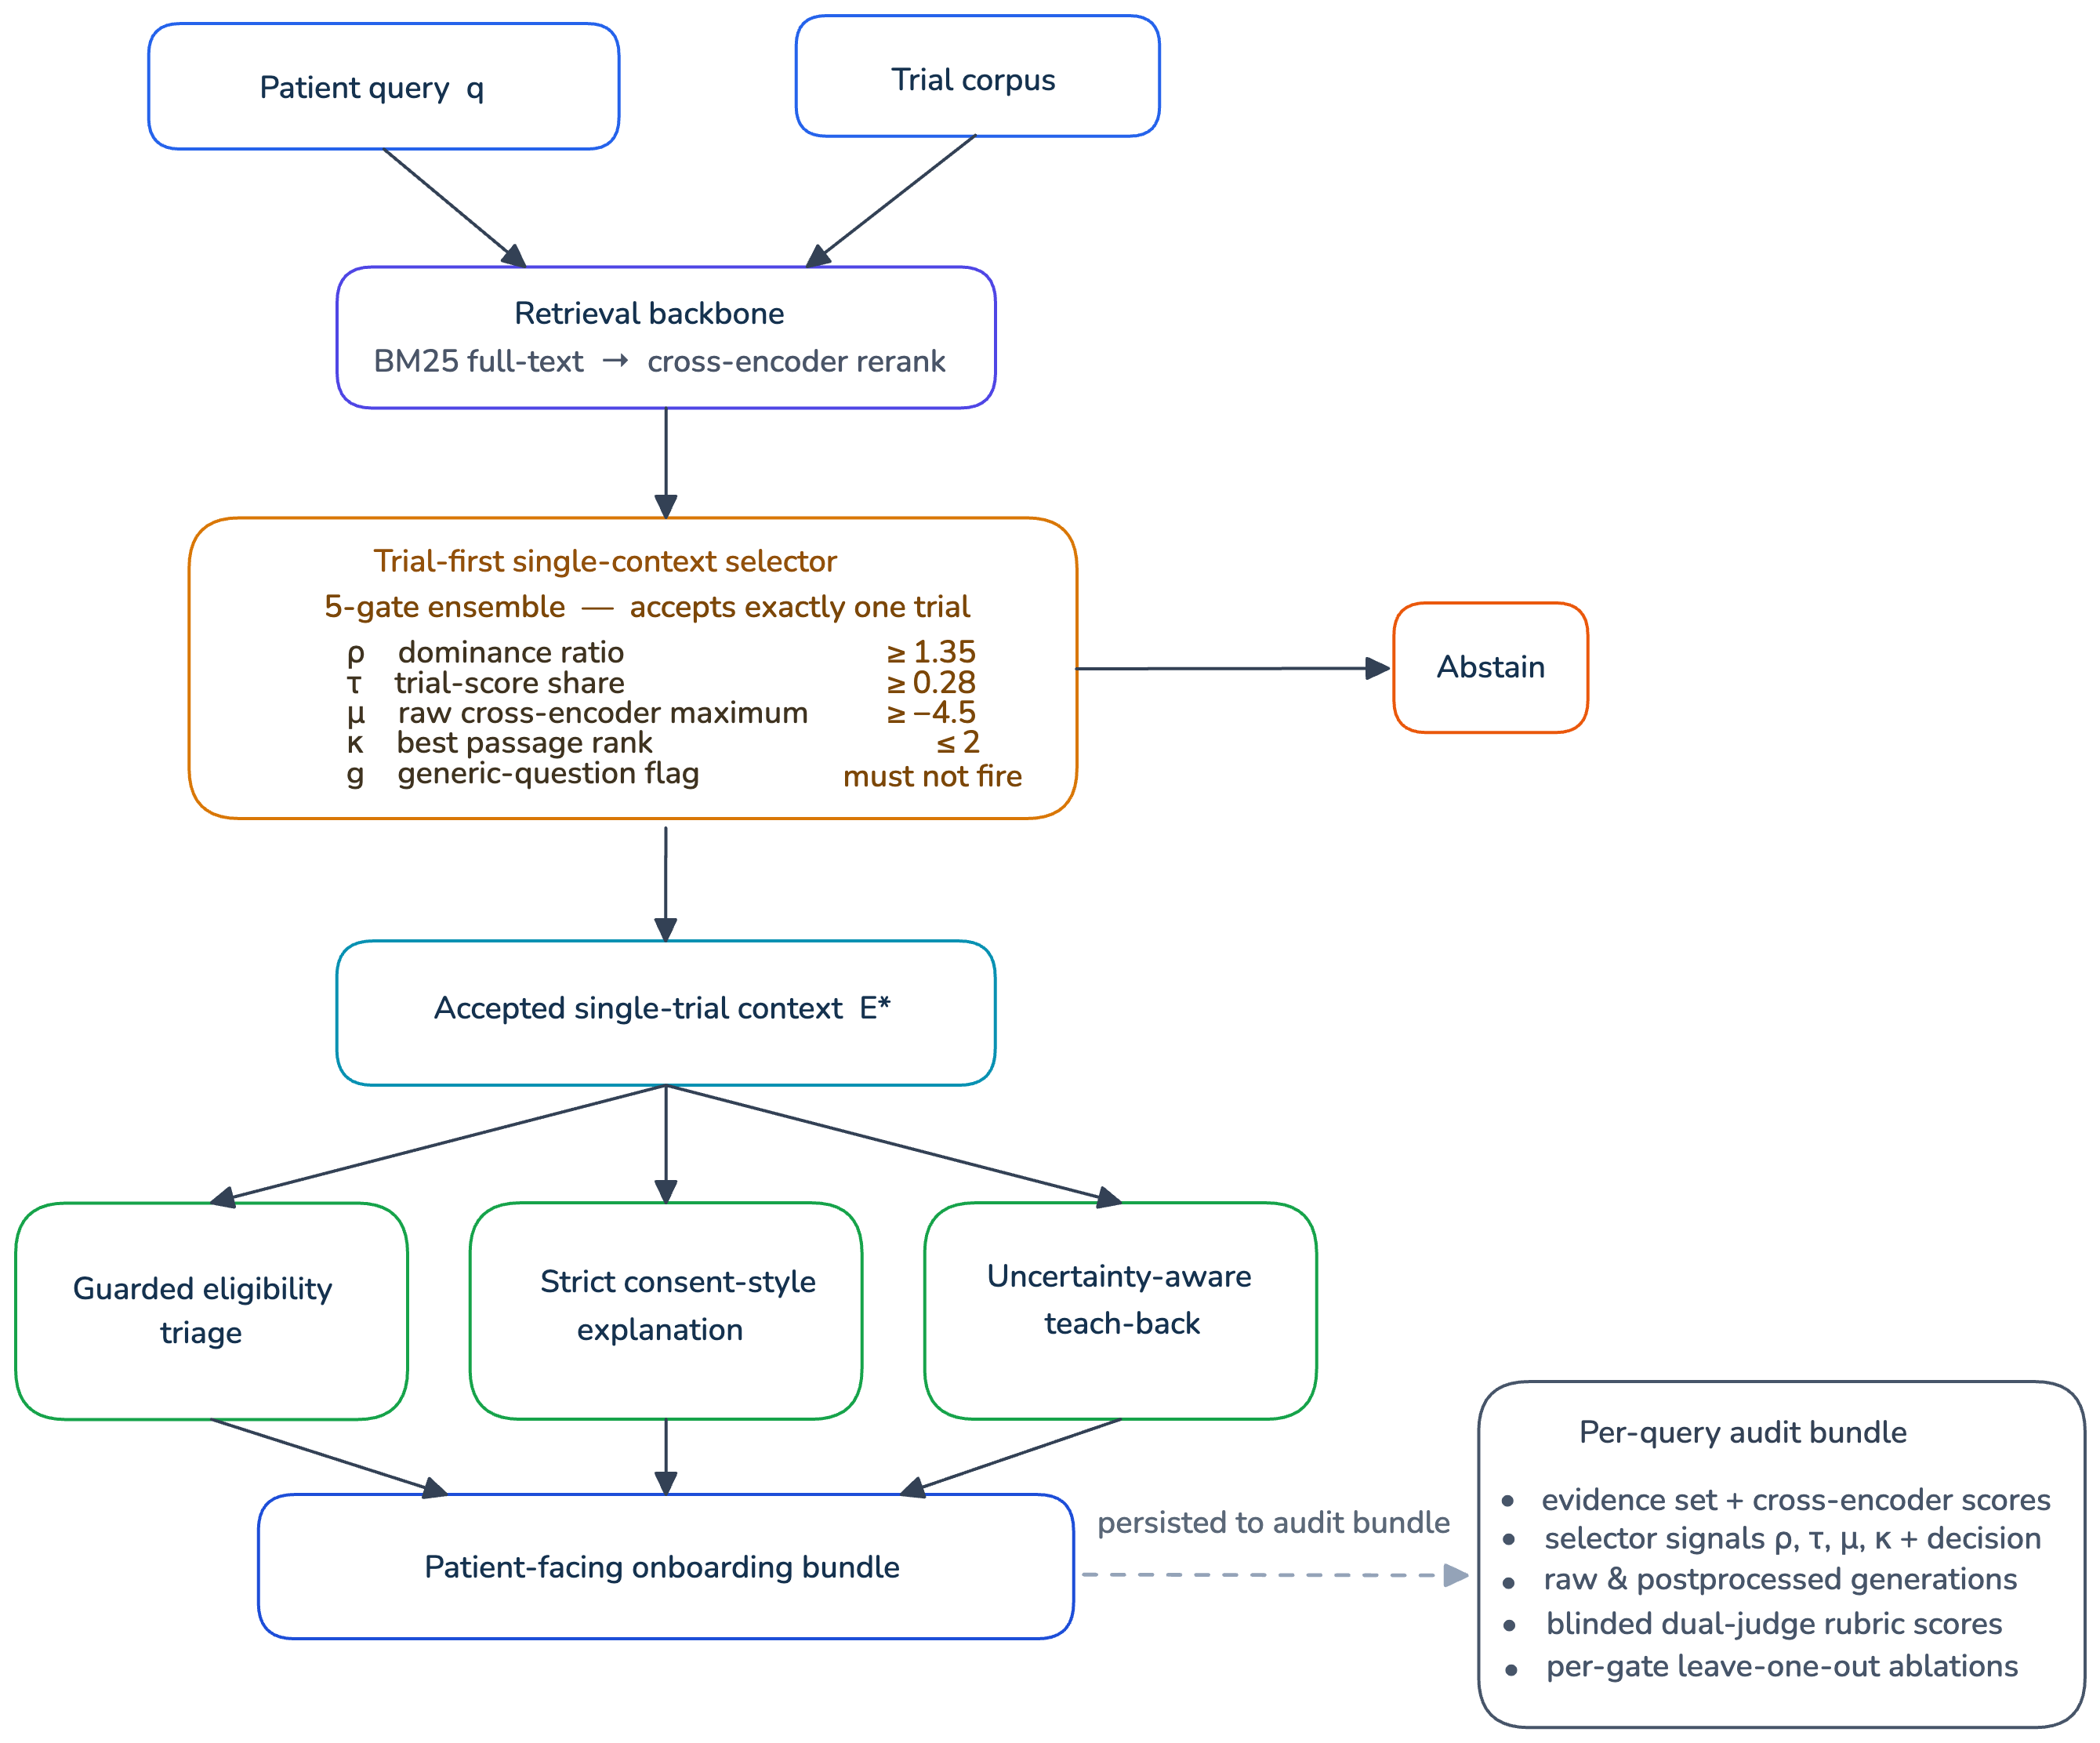
\includegraphics[width=0.96\linewidth]{figures/pipeline_architecture.png}
\caption{\textbf{Grounded clinical trial onboarding pipeline.} A patient query and the trial corpus enter the retrieval backbone (BM25 full-text $\to$ cross-encoder reranking). The trial-first selector accepts a single dominant trial only if its dominance ratio $\rho$, score share $\tau$, raw cross-encoder maximum $\mu$, and best rank $\kappa$ clear configured thresholds and the query is not flagged generic; otherwise the pipeline abstains with a narrowing prompt. Downstream modules---guarded eligibility triage, strict consent-style explanation with evidence-bounded fallback, and uncertainty-aware teach-back---all draw from the same accepted trial. Audit artifacts are persisted per query.}
\label{fig:pipeline}
\end{figure}

% ============================================================
\section{Related Work}
\label{sec:related}

\subsection{Patient--trial matching and recruitment}
Early patient--trial matching systems relied on structured embeddings and entailment over criteria text \citep{zhang2020deepenroll,gao2020compose,bustos2018trial}. More recent work applies LLMs either as criterion-level reasoners (\emph{TrialGPT} \citep{jin2024trialgpt}), as semantic matchers over patient records (\emph{PRISM} \citep{gupta2024prism}), or at enterprise scale in oncology \citep{wong2024scaling,nievas2024distilling}. Closely related work further extends this line to fairness \citep{chang2024fair}, recruitment and retention \citep{lu2024airecruit,unger2019recruitment,clark2019barriers}, zero-shot trial similarity \citep{wang2023trial2vec}, and cancer-informatics matching at scale \citep{chen2025enhancing}. Unlike these systems, our work does not optimize for match accuracy as the primary objective. Instead, it treats matching as \emph{only one} of several onboarding outputs, and pairs it with an explanation module and a teach-back module to make the interaction auditable and patient-facing.

\subsection{Retrieval-augmented generation and medical RAG}
RAG \citep{lewis2020rag,guu2020realm,karpukhin2020dpr,izacard2022contriever,reimers2019sbert,thakur2021beir} has become a standard strategy for grounding LLMs on external knowledge. In healthcare, RAG has been used to build clinical copilots \citep{zhao2025medrag}, benchmark medical information retrieval \citep{xiong2024benchmarking}, and summarize systematic evidence \citep{neha2025ragsystematic,maity2025llmhealth}. Lexical baselines such as \textsc{BM25} \citep{robertson2009bm25} remain competitive on heterogeneous benchmarks \citep{thakur2021beir,lin2021pyserini}, especially when paired with cross-encoder reranking \citep{nogueira2019passage,khattab2020colbert,hofstatter2021crossenc,wang2020minilm}. Dense retrievers such as Sentence-BERT, DPR, Contriever, and BGE \citep{reimers2019sbert,karpukhin2020dpr,izacard2022contriever,xiao2024bge} improve semantic coverage but can lose recall on long, heterogeneous documents, which is consistent with our own findings on trial text.

\subsection{Safety, hallucination, and uncertainty in clinical NLP}
Hallucination and factual faithfulness remain central challenges for generative models \citep{ji2023hallucination,maynez2020faithfulness,huang2025survey,min2023factscore}, and are particularly acute in medical question answering \citep{pal2023medhalu,ayers2023comparing,lievin2024can}. Recent work on uncertainty estimation and calibration for medical LLMs \citep{wu2024uncertainty,zhou2025uncertaintyaware,wang2025trustworthy,lucas2024reasoning,kadavath2022know,mielke2022reducing} has explored verifiable abstention, linguistic calibration, and explainability. Prior foundational biomedical models \citep{lee2020biobert,alsentzer2019clinicalbert} established domain-specific representations that inform much of this literature. Our design complements these directions: rather than only calibrating token-level confidence, we enforce \emph{structural} uncertainty through evidence-bounded fallback fields and a trial-first context gate.

\subsection{Informed consent, teach-back, and patient-facing communication}
Teach-back and related strategies are well-supported interventions for improving comprehension of informed-consent information and for research participation in lower-literacy settings \citep{kripalani2008teachback,talevski2020teachback,kadam2017informed,jamerson2023evaluation,tamariz2013improving,glaser2020interventions,burks2019health,ho2017teachback,sudore2009interventions}. Patient-centered language processing is an emerging focus within NLP, exemplified by patient-voiced eligibility reasoning \citep{aguiar2025amieligible,chen2025enhancing}. Our teach-back module differs from prior patient-education work in that its questions are not templated from generic consent forms but are conditioned on the pipeline's \emph{own} identified uncertainties, so the educational loop probes exactly the concepts the system could not verify.

\subsection{Clinical deployment and equity considerations}
Safe deployment of AI systems in clinical contexts raises concerns about representativeness, bias, and reliability \citep{obermeyer2019dissecting,wornow2023shaky,topol2019deep,fda2022diversity,clark2019barriers,weng2017medical,spasic2020clinical}. Our system does not claim to replace study-team screening or formal consent; it is designed explicitly as a pre-screening communication aid with audit artifacts for every response.

% ============================================================
\section{Results}
\label{sec:results}

\subsection{Headline safety result: zero detected lexical cross-trial leakage under the audited conditions; residual semantic leakage quantified}
\label{sec:results_leak}

Across all 114 onboarding cases, all six model families, both selector regimes, and both pre-specified \emph{lexical} leak definitions, the cross-trial leak rate was $0\%$ (Table~\ref{tab:six_backbone}; per-cell heatmap in Supplementary Information \S~5). The narrow definition flagged any \texttt{NCT}-identifier other than the selected trial in any model-emitted text field; the wide definition additionally matched distinctive non-stop title tokens unique to a single non-selected trial. Both produced identical rates: $0/684$ generations.

To stress-test for the residual channel of \emph{paraphrased} cross-trial content that no lexical detector can catch by construction (reviewer-2's concern), we add a third pre-specified \textbf{semantic LLM-judge detector}: each generation is independently scored by Claude Sonnet~4.5 and GPT-4o under a structured rubric that returns a binary \texttt{semantic\_leak} flag plus the suspect non-selected trial, a $\leq 250$-char verbatim claim excerpt, and a two-sentence rationale (prompt in Supplementary \S2.6). Across the 684-generation audit, the semantic detector flags $12/684 = 1.75\%$ under the conservative \emph{both-judges-agree} consensus (Cohen $\kappa = 0.16$; raw agreement $86.5\%$; pooled either-judge rate $104/684 = 15.2\%$); the low $\kappa$ despite high raw agreement reflects the rarity of consensus flags (prevalence imbalance), the same kappa-paradox mechanism discussed in \S\ref{sec:results_irr_brief}, rather than judge instability. Manual review of all $12$ consensus-flagged cases classifies $8$ as unambiguous paraphrased cross-trial content (e.g., a HER2-positive eligibility claim asserted for a HER2-negative selected trial; a one-year-post-pituitary-surgery exclusion attributed to a trial whose criteria do not contain it; a continued-octreotide-LAR treatment plan asserted for a selected trial that describes only surgical resection), $2$ as mixed cases where the answer contains a model error whose attribution to a specific non-selected trial is ambiguous (the two judges name different suspect trials, or the hallucinated content is not traceable to any single pool trial), and $2$ as likely judge over-interpretation of generic clinical English that also fits the selected trial. The per-backbone consensus rate is reported in the rightmost column of Table~\ref{tab:six_backbone}; the largest residual sits on the smallest open-weight backbone (Qwen-2.5-3B at $3.51\%$), the smallest on the closed-API baselines ($0.88\%$ each). All twelve consensus-flagged cases pass the lexical detectors (no \texttt{NCT}-id, no distinctive vocabulary), confirming that semantic and lexical layers test orthogonal channels.

\begin{table}[!htbp]
\centering
\caption{\textbf{Six-backbone safety summary on the $n=114$ pool} ($684$ generations total). Closed-API baselines (GPT-4o, Claude Sonnet~4.5) are zero-shot with our identical guarded evidence and JSON-schema prompt; no fine-tuning. Leak rate is zero for every model under both lexical definitions; the rightmost column reports the third semantic detector under conservative both-judges-agree consensus. Leak$_{\mathrm{nar}}$: narrow \texttt{NCT}-identifier regex; Leak$_{\mathrm{wide}}$: wide entity-resolved match; Leak$_{\mathrm{sem}}$: semantic dual-judge consensus. (cand.): low-latency deployment-candidate backbone; the system is not clinically deployed.}
\label{tab:six_backbone}
\small
\setlength{\tabcolsep}{4pt}
\begin{tabular}{lcccccccc}
\toprule
Model & Family & $N$ & Parse-ok & Commit & Abstain & Leak$_{\mathrm{nar}}$ & Leak$_{\mathrm{wide}}$ & Leak$_{\mathrm{sem}}$ \\
\midrule
Qwen-2.5-3B (cand.) & open-weight & 114 & 0.63 & 0.55 & 0.00 & \textbf{0.00} & \textbf{0.00} & 0.035 \\
Qwen-2.5-7B        & open-weight & 114 & 0.89 & 0.44 & 0.00 & \textbf{0.00} & \textbf{0.00} & 0.018 \\
Meta-Llama-3.1-8B  & open-weight & 114 & 0.39 & 0.19 & 0.00 & \textbf{0.00} & \textbf{0.00} & 0.018 \\
Mistral-7B-v0.3    & open-weight & 114 & 0.12 & 0.11 & 0.01 & \textbf{0.00} & \textbf{0.00} & 0.018 \\
GPT-4o             & closed-API  & 114 & \textbf{1.00} & 0.31 & 0.04 & \textbf{0.00} & --- & \textbf{0.009} \\
Claude Sonnet~4.5  & closed-API  & 114 & \textbf{1.00} & 0.14 & 0.11 & \textbf{0.00} & --- & \textbf{0.009} \\
\bottomrule
\end{tabular}
\end{table}

The result holds across the six therapeutic-area strata of the case pool (musculoskeletal, cardiovascular, metabolic / endocrine, oncology, neurology / CNS, and a heterogeneous \emph{Other} bucket; Fig.~\ref{fig:per_area}). Every one of the 24 (area $\times$ open-weight backbone) cells has leak rate $0$; commit and parse-ok rates track the per-backbone fluency hierarchy already evident in Table~\ref{tab:six_backbone}.

\begin{figure}[!htbp]
\centering
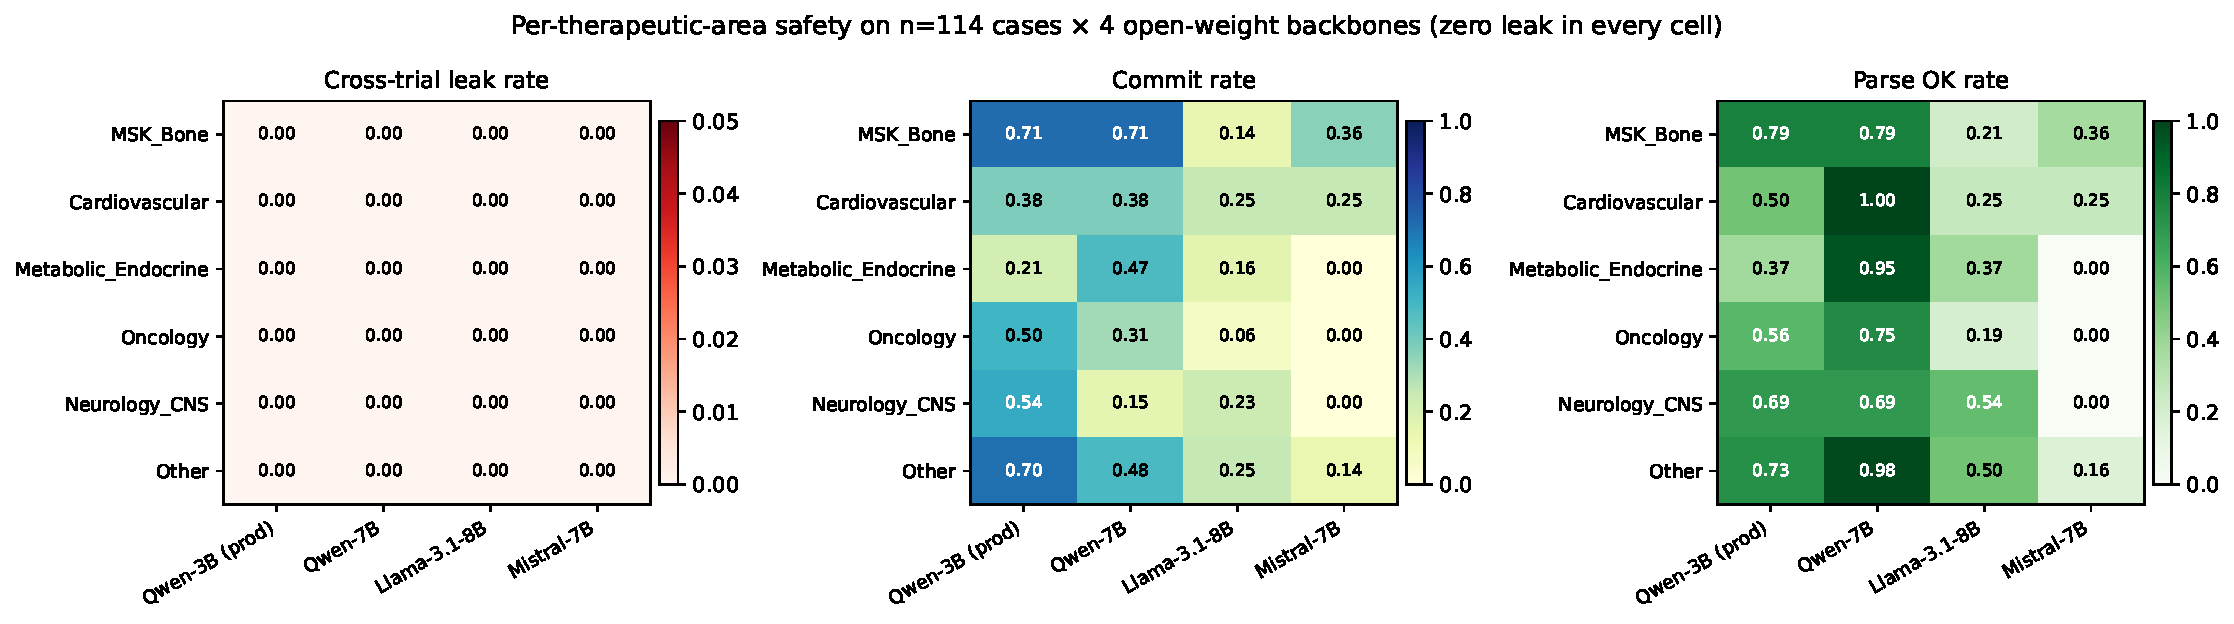
\includegraphics[width=0.96\linewidth]{figures/per_area_heatmap.pdf}
\caption{\textbf{Per-(therapeutic area $\times$ backbone) behavior on $n=114$ open-weight cases.} Left: cross-trial leak rate---uniformly $0$ in every cell. Center: commit rate. Right: parse-ok rate. Per-area commit and parse-ok track the per-backbone fluency hierarchy; the safety property is preserved across all six therapeutic areas tested.}
\label{fig:per_area}
\end{figure}

\subsection{Per-gate ablation: no single gate is solely responsible for zero lexical leak}
\label{sec:results_pergate}

A reviewer-facing question is whether any single gate is solely responsible for the zero-lexical-leak property. We ran a leave-one-out counterfactual ablation in which each gate is dropped while the others remain active (Methods, \S\ref{sec:methods_pergate}). Three variants admit additional cases relative to the deployed configuration: dropping $\mu$ admits 27 additional cases, dropping $\rho$ admits 10, and dropping the generic-flag admits 6. Two variants---no-$\tau$ and no-$\kappa$---admit zero additional cases under the deployed thresholds, indicating these gates are slack: every case rejected by $\tau$ or $\kappa$ alone is also rejected by at least one other gate. Despite the broader admission under the relaxed variants, leak rate remained $0$ in every (variant $\times$ backbone) cell (Table~\ref{tab:per_gate}). The safety property therefore resides in the gate ensemble as a whole, not in any single condition.

\begin{table}[!htbp]
\centering
\caption{\textbf{Counterfactual leave-one-out per-gate ablation on $n=114$.} Each variant relaxes one accept condition while the others remain active. ``Only this gate'' counts cases admitted by the variant that the deployed configuration rejected. Leak rate is $0$ in every (variant $\times$ backbone) cell.}
\label{tab:per_gate}
\small
\setlength{\tabcolsep}{4pt}
\begin{tabular}{l c c | c c c c}
\toprule
Variant & \makecell[c]{Accepted\\(of $n{=}114$)} & \makecell[c]{Only\\this gate} & \multicolumn{4}{c}{Leak rate per backbone} \\
& & & Qwen-2.5-3B & Qwen-2.5-7B & Llama-8B & Mistral-7B \\
\midrule
deployed             & 32 & --- & 0.00 & 0.00 & 0.00 & 0.00 \\
no-$\rho$            & 42 & 10 & 0.00 & 0.00 & 0.00 & 0.00 \\
no-$\tau$            & 32 & 0  & 0.00 & 0.00 & 0.00 & 0.00 \\
no-$\mu$             & 59 & 27 & 0.00 & 0.00 & 0.00 & 0.00 \\
no-$\kappa$          & 32 & 0  & 0.00 & 0.00 & 0.00 & 0.00 \\
no-generic           & 38 & 6  & 0.00 & 0.00 & 0.00 & 0.00 \\
\bottomrule
\end{tabular}
\end{table}

\subsection{Adversarial subset audit: where in the case pool does residual semantic leakage concentrate?}
\label{sec:results_adversarial}

A natural reviewer question is whether the residual semantic-detector signal is uniformly distributed across the audited pool or concentrated in cases where the retrieval pool is structurally ambiguous. We pre-defined the \emph{adversarial subset} as cases with selector dominance ratio $\rho < 1.5$ \emph{and} $\geq 2$ distinct trials in the candidate pool---i.e., cases where the gate ensemble is closest to abstaining and where cross-trial conflation is most plausible. This yields 53 of 114 cases ($46.5\%$); the remaining 61 are the non-adversarial subset. We stratify the four open-weight backbones across the two subsets (closed-API baselines are excluded from this analysis because the existing wide-leak detector does not apply, so the lexical comparison is not on the same footing) and compare detector rates per stratum (Table~\ref{tab:adv_subset}).

\begin{table}[!htbp]
\centering
\caption{\textbf{Adversarial-subset stratification of the 456 open-weight (case $\times$ backbone) cells.} The adversarial subset is defined pre-hoc as dominance ratio $\rho < 1.5$ and $\geq 2$ trials in the candidate pool. Lexical detectors (narrow + wide) flag no leakage in either stratum. The semantic detector's conservative both-judges-agree rate is $\sim 3$--$5\times$ higher in the adversarial subset than in the non-adversarial subset and is concentrated on the smallest backbone (Qwen-2.5-3B). Either-judge rates in parentheses.}
\label{tab:adv_subset}
\small
\setlength{\tabcolsep}{4pt}
\begin{tabular}{l c c c c c}
\toprule
Backbone & Stratum & $n$ & Narrow & Wide & Sem-both (Sem-either) \\
\midrule
Qwen-2.5-3B   & non-adversarial & 61 & 0.00 & 0.00 & 0.016 (0.115) \\
Qwen-2.5-3B   & \textbf{adversarial} & 53 & 0.00 & 0.00 & \textbf{0.057} (0.302) \\
\midrule
Qwen-2.5-7B   & non-adversarial & 61 & 0.00 & 0.00 & 0.000 (0.131) \\
Qwen-2.5-7B   & \textbf{adversarial} & 53 & 0.00 & 0.00 & \textbf{0.038} (0.170) \\
\midrule
Llama-3.1-8B  & non-adversarial & 61 & 0.00 & 0.00 & 0.000 (0.082) \\
Llama-3.1-8B  & \textbf{adversarial} & 53 & 0.00 & 0.00 & \textbf{0.038} (0.151) \\
\midrule
Mistral-7B    & non-adversarial & 61 & 0.00 & 0.00 & 0.016 (0.180) \\
Mistral-7B    & \textbf{adversarial} & 53 & 0.00 & 0.00 & \textbf{0.019} (0.321) \\
\bottomrule
\end{tabular}
\end{table}

The pattern is consistent with the design intent of the gate ensemble: the lexical safety property is fully preserved on the adversarial subset (zero leak under narrow and wide detectors), while the third semantic detector localizes the residual paraphrase-leakage signal precisely to the cases that are structurally hardest for a single-trial guard. The strongest residual sits on Qwen-2.5-3B ($5.7\%$ adversarial vs.\ $1.6\%$ non-adversarial); the deployment guidance is therefore to either escalate the abstain-prompt threshold on cases with $\rho < 1.5$ or to add the claim-level natural-language-inference (NLI) verification step we evaluate in \S\ref{sec:results_nli}.

\subsection{Baseline comparison: only structural single-trial control closes the cross-trial channel}
\label{sec:results_baselines}

A central reviewer question is whether the safety property requires the structural single-trial guard at all, or whether a simpler intervention---standard retrieval-augmented generation, a prompt-only instruction, citation enforcement, or trivial top-1 selection---would suffice. We therefore evaluated four pre-registered baselines on the same $n=114$ pool and the two deployment backbones (Qwen-2.5-7B, Qwen-2.5-3B; $912$ generations), holding the retrieval, prompt scaffold, and post-processor fixed and changing only the evidence-control mechanism (Methods, \S\ref{sec:methods_baselines}): \textbf{B1} standard multi-trial RAG (top-6 passages across trials, no guard); \textbf{B2} the same evidence plus a strong prompt-only anti-mixing instruction; \textbf{B3} citation-enforced generation (every field must cite passage identifiers; uncited fields are dropped); and \textbf{B4} trivial top-1 selection (the trial owning the rank-1 passage, no five-gate ensemble). All baselines are audited by the identical three detectors (narrow + wide lexical, dual-judge semantic) used for V-final.

The contrast is decisive (Table~\ref{tab:baselines}; Fig.~\ref{fig:baseline_leak}). The two multi-trial-evidence baselines and the citation-enforced baseline leak heavily: under the conservative both-judges-agree semantic consensus, B1 reaches $58.3\%$, B2 $50.9\%$, and B3 $59.0\%$; their lexical wide-leak rates are $2.2\%$, $5.3\%$, and $21.1\%$ respectively. Prompt-only mitigation (B2) does not close the channel, and citation enforcement (B3) is the \emph{worst} configuration on the lexical axis---requiring the generator to cite passages surfaces multi-trial content rather than suppressing it (the $7$B model cites cross-trial passages in $41\%$ of cases). In sharp contrast, the structural single-trial baselines match the deployed pipeline: B4 top-1 selection has $0\%$ lexical leak and $1.3\%$ semantic-consensus leak, indistinguishable from V-final's $0\%$ lexical and $1.8\%$ semantic consensus. The single-trial \emph{structural} property---not the prompt, not citation enforcement---is what closes the channel.

\begin{table}[!htbp]
\centering
\caption{\textbf{Four-baseline comparison on the $n=114$ pool ($912$ generations) vs.\ the deployed V-final pipeline.} Lexical = wide entity-resolved detector; Semantic = both-judges-agree (Sonnet~4.5 + GPT-4o) consensus. Taxonomy columns count consensus-flagged generations by category (T1 cross-trial contamination, T2 unsupported clinical completion, T3 ordinary hallucination). Only structural single-trial control (B4, V-final) drives both channels near zero and eliminates T1 entirely.}
\label{tab:baselines}
\small
\setlength{\tabcolsep}{5pt}
\begin{tabular}{l c c c c c}
\toprule
System & Lexical (wide) & Semantic (consensus) & T1 & T2 & T3 \\
\midrule
V-final (single-trial guard) & \textbf{0.000} & \textbf{0.018} & --- & --- & --- \\
B1: multi-trial RAG          & 0.022 & 0.583 & 124 & 9 & 0 \\
B2: prompt-only guard        & 0.053 & 0.509 & 107 & 8 & 0 \\
B3: citation-enforced        & 0.211 & 0.590 & 125 & 9 & 0 \\
B4: top-1 selection          & \textbf{0.000} & \textbf{0.013} & \textbf{0} & 2 & 1 \\
\bottomrule
\end{tabular}
\end{table}

\begin{figure}[!htbp]
\centering
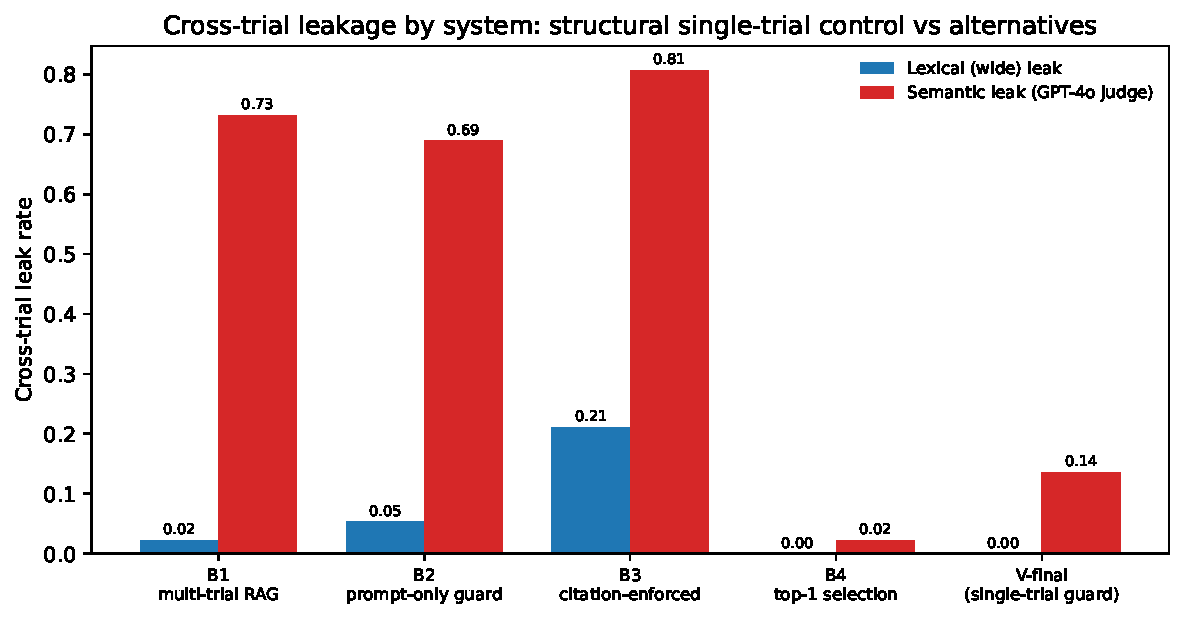
\includegraphics[width=0.92\linewidth]{figures/phase5_baseline_leak_bars.pdf}
\caption{\textbf{Cross-trial leakage by system.} Lexical (wide) and dual-judge-consensus semantic leak rates for the four baselines and the deployed V-final pipeline. Multi-trial RAG, prompt-only guarding, and citation enforcement all leak; structural single-trial control (B4 top-1, V-final) closes both channels.}
\label{fig:baseline_leak}
\end{figure}

\subsection{Failure taxonomy: structural control removes contamination, not generator-level error}
\label{sec:results_taxonomy}

To separate the safety problem this paper targets from adjacent failure modes, we classify every consensus-flagged generation into three mutually exclusive categories, defined in Methods \S\ref{sec:methods_taxonomy}: \textbf{T1 cross-trial contamination} (a claim supported only by a non-selected trial in the retrieval pool); \textbf{T2 unsupported clinical completion} (plausible protocol-style content supported by no pool trial); and \textbf{T3 ordinary hallucination} (a claim false on its face or incoherent with the case). This distinction is itself a contribution: cross-trial conflation (T1) is an evidence-layer property that structural control can eliminate, whereas T2/T3 are generator-level errors that single-trial control is not designed to remove.

The taxonomy makes the mechanism explicit (Table~\ref{tab:baselines}; Fig.~\ref{fig:taxonomy}). For the multi-trial baselines B1--B3, the consensus-flagged failures are overwhelmingly T1 ($107$--$125$ of each), confirming that their leakage is genuine cross-trial contamination. For B4 top-1 selection, T1 falls to \emph{zero}: its handful of residual flags are T2 ($2$) and T3 ($1$)---generator-level errors that no evidence-layer guard removes. Structural single-trial control therefore eliminates exactly the failure class it targets, and the residual on guarded systems is a different, smaller problem (unsupported completion), which motivates the claim-level verification step below.

\begin{figure}[!htbp]
\centering
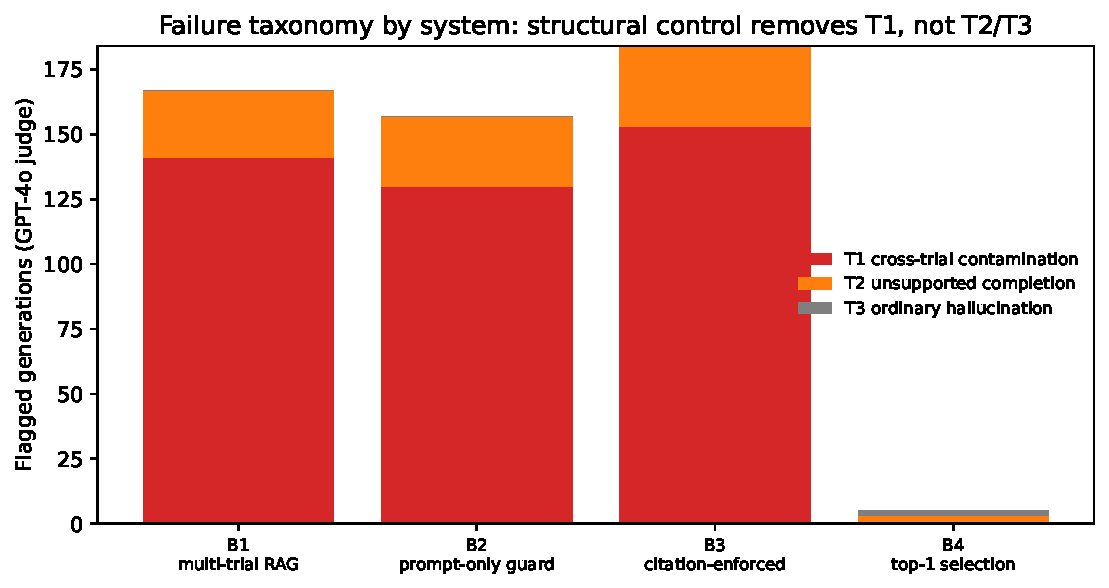
\includegraphics[width=0.82\linewidth]{figures/phase5_taxonomy_breakdown.pdf}
\caption{\textbf{Failure taxonomy by system.} Consensus-flagged generations partitioned into T1 cross-trial contamination, T2 unsupported completion, and T3 ordinary hallucination. Multi-trial baselines are T1-dominated; structural top-1 control removes T1 entirely, leaving only generator-level T2/T3.}
\label{fig:taxonomy}
\end{figure}

\subsection{Claim-level NLI verification reduces the residual semantic channel}
\label{sec:results_nli}

The residual paraphrased-semantic channel (Theorem~\ref{thm:safety} boundary iv) is the one channel structural control does not close by construction. We implement and evaluate the claim-level verification step the original manuscript only proposed: a natural-language-inference (NLI) post-processor (DeBERTa-v3-large MNLI) that, for every asserted patient-facing claim, compares entailment by the selected trial's evidence ($e_{\mathrm{sel}}$) against the maximum entailment by any non-selected pool trial ($e_{\mathrm{other}}$), and redacts a claim when $e_{\mathrm{other}} \ge \tau_{\mathrm{NLI}}$ and $e_{\mathrm{other}} > e_{\mathrm{sel}}$---i.e., precisely when a competing trial supports the claim better than the selected one (Methods, \S\ref{sec:methods_nli}). The threshold $\tau_{\mathrm{NLI}}=0.95$ was fixed on the 15-case development pool alone (highest threshold with development benign-drop $\le 10\%$), before any application to the audit pool.

Applied to the frozen 684-generation audit, the verifier redacts $8$ of the $12$ both-judges-consensus semantic leaks---exactly the eight that manual review had classified as unambiguous cross-trial content; the four it correctly retains are the two mixed-attribution model errors and the two judge over-flags that are not in fact cross-trial. The utility cost is modest and quantified: $15.1\%$ of asserted claims are dropped overall ($17.9\%$ on the accept regime, $14.1\%$ on the abstain regime), trading a fraction of generic pool-shared claims for closure of the genuine cross-trial channel. This converts Theorem~\ref{thm:safety} boundary (iv) from a proposed mitigation into an evaluated one and is the recommended hardening for the smallest backbone, where the residual concentrates.

\subsection{Safety is invariant to the backbone; fluency is not}
\label{sec:results_backbone_gate}

Leak rate is uniform across the six families, but parse-ok, commit, and per-case latency vary substantially (Table~\ref{tab:six_backbone}). To locate the safety property, we computed Spearman rank correlations between the four continuous selector signals and the per-case judge-pooled rubric scores, stratified by backbone (Supplementary Fig.~S11). The weaker backbones inherit fluency from the evidence: Mistral-7B and Llama-3.1-8B show moderate positive coupling between the raw cross-encoder maximum $\mu$ and factuality (Mistral: $r_s = 0.51$, $p < 0.01$; Llama: $r_s = 0.36$, $p < 0.05$) and between $\mu$ and groundedness (Mistral: $r_s = 0.53$, $p < 0.01$)---they are more factual when the reranker strongly supports the top trial, and drift when it does not. For the stronger Qwen-2.5-7B, signal--rubric correlations collapse, as expected for a guard-and-generator pair where the guard has already filtered the evidence. None of these per-backbone differences in fluency or signal sensitivity translate into different leak rates: the gate ensemble forces every backbone onto the same single-trial evidence pool, and the leak channel is closed by construction (Theorem~\ref{thm:safety}).

\subsection{Abstain-regime behavior: the system stays safe and useful when no single trial dominates}
\label{sec:results_abstain}

Real-world onboarding queries frequently fall into the abstain regime---no single dominant trial in the candidate pool (e.g., ``I had some bone problems''). To address this directly, the dual-judge protocol scored every generation on the 82 abstain-regime cases probed with the gate disabled. The narrowing-prompt response (``I could not identify one reliable study; please share the study title or NCT number'') is itself a safe and patient-facing output even when the system declines to commit. As a consequence, the abstain-regime safety score sits at or above $4.0/5$ for every backbone, and the abstain-regime overall rubric mean is comparable to or higher than the accept-regime mean for the three top backbones (Fig.~\ref{fig:abstain}; Supplementary Table~S12). The system does not gamble on weakly grounded commits to remain useful. Operationally, abstention is a workflow feature rather than a failure mode: the narrowing prompt elicits the study title or \texttt{NCT} number from the patient, improving the quality of the next interaction turn, and it avoids exposing the patient to weakly grounded eligibility content that a coordinator would later need to correct.

To quantify what abstention actually costs, we measured how often a relevant trial was in fact available in the candidate pool of an abstained case---i.e., a missed-utility opportunity. Across the 82 abstain-regime cases, only $18$ ($22.0\%$; Clopper--Pearson 95\% CI $13.6$--$32.5\%$) had a qrels-relevant trial present in the retrieved pool, while $64$ ($78.0\%$) had no relevant trial available, meaning abstention was the correct action. The high abstention rate is therefore dominated by cases where committing would have been unsafe, not by discarded opportunities. The safety--utility trade-off across all five systems is summarized in Fig.~\ref{fig:frontier}: the structural single-trial systems (B4 top-1 and V-final) occupy the low-leak region, and B4 attains the highest GPT-4o rubric utility ($4.21/5$) of any baseline while holding leakage near zero---structural control is Pareto-favourable rather than a safety-for-utility trade.

\begin{figure}[!htbp]
\centering
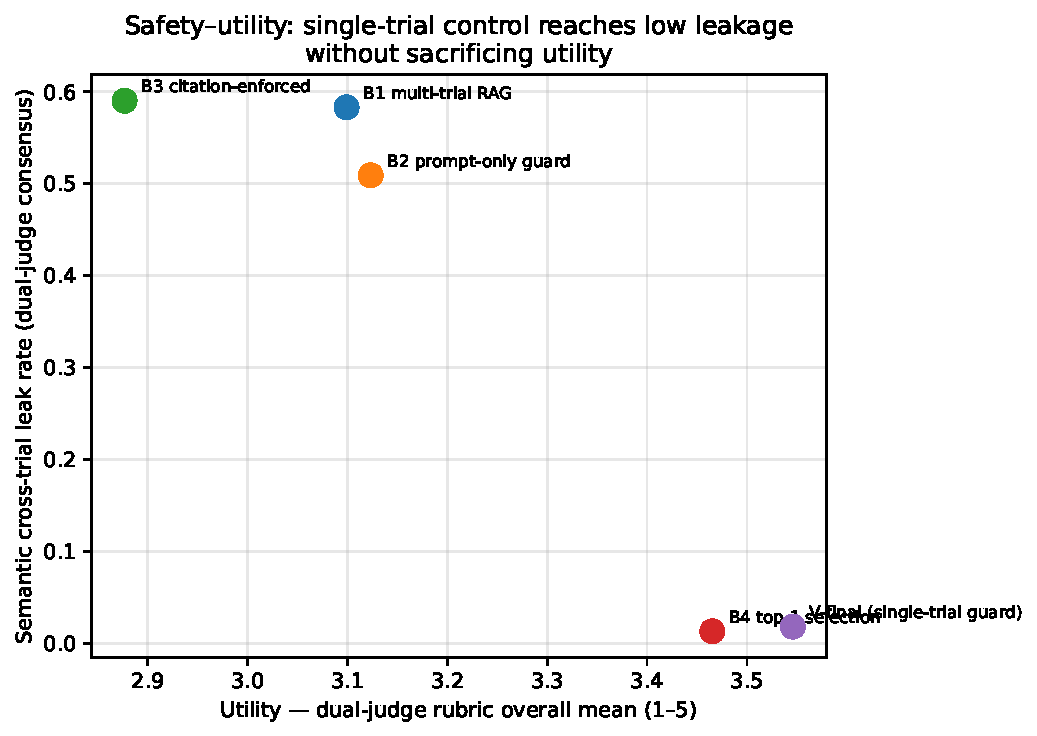
\includegraphics[width=0.80\linewidth]{figures/phase5_safety_utility_frontier.pdf}
\caption{\textbf{Safety--utility trade-off across systems.} $x$-axis: utility (rubric overall mean; baselines scored by GPT-4o, V-final by the dual-judge pool over the harder full $n=114$ regime). $y$-axis: dual-judge-consensus semantic leak rate. Only the structural single-trial systems (B4, V-final) reach the low-leak region; B4 does so at the highest baseline utility.}
\label{fig:frontier}
\end{figure}

\begin{figure}[!htbp]
\centering
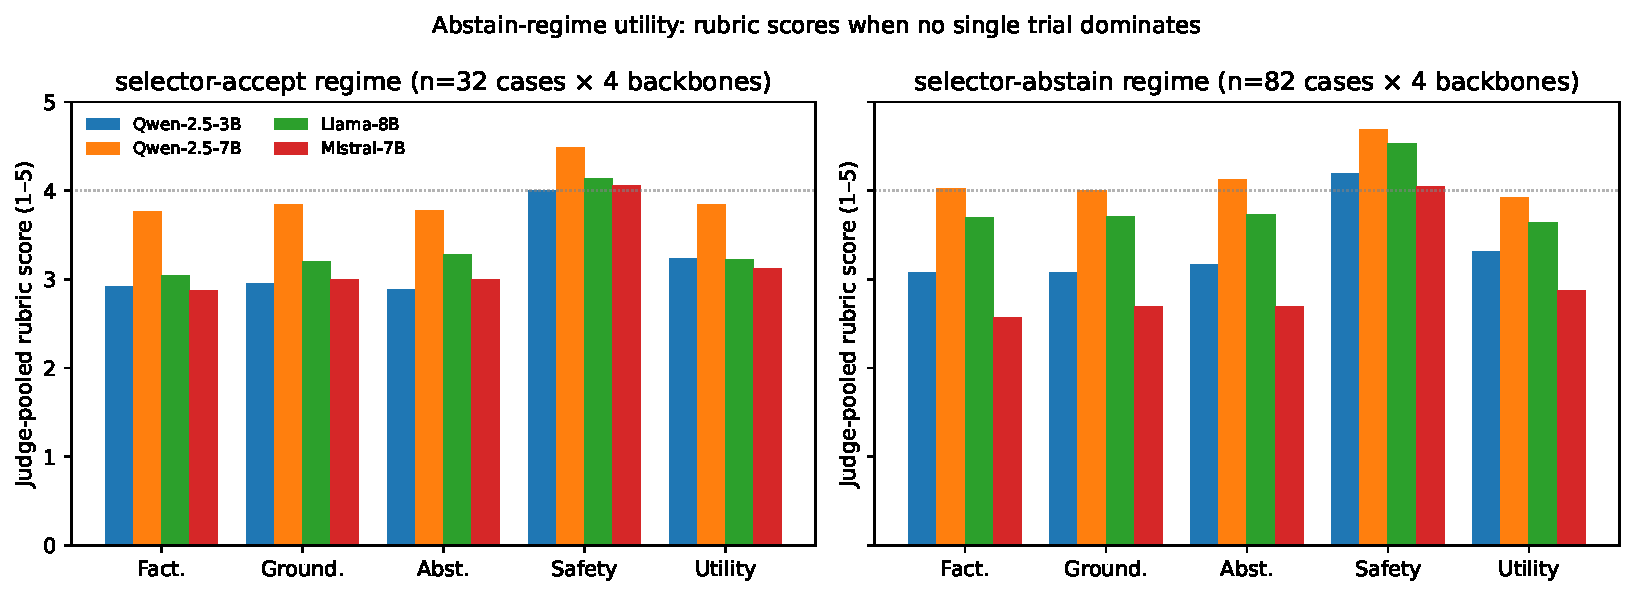
\includegraphics[width=0.96\linewidth]{figures/abstain_regime_quality.pdf}
\caption{\textbf{Abstain-regime utility: judge-pooled rubric scores per (regime, backbone).} Safety remains at the elevated ceiling in both regimes; overall fluency is comparable or higher in the abstain regime for three of four backbones, because the narrowing prompt is itself a high-quality patient-facing output.}
\label{fig:abstain}
\end{figure}

\subsection{Blind dual-judge LLM evaluation}
\label{sec:results_judge}

Two LLM judges (Claude Sonnet~4.5, GPT-4o) blind-scored all 684 generations on a five-dimension rubric (factuality, groundedness, abstention appropriateness, safety, patient utility; 1--5 scale). The blinding protocol is detailed in Methods, \S\ref{sec:methods_judge}; in brief, judges received a SHA1 \texttt{blind\_id}, a per-judge case-shuffled ordering, and a normalized JavaScript Object Notation (JSON) output (no raw decoder text or model-specific verbose styles). Qwen-2.5-7B led on every dimension with overall mean $3.95$ (95\% bootstrap confidence interval (CI) $[3.76, 4.14]$); the deployment-candidate Qwen-2.5-3B reached a comparable safety level ($4.14$ vs.\ $4.63$) at $44\%$ lower mean latency ($11.0$ vs.\ $19.8$ s), which is the deployment trade-off we accept. Inter-judge agreement was moderate on the substantive dimensions (Spearman rank correlation $r_s \in [0.52, 0.56]$ for factuality / groundedness / patient utility) and ceiling-bound on safety and calibration-subjective on abstention (\S\ref{sec:results_irr_brief}). The full per-backbone rubric table at $n=114$ with bootstrap 95\% CIs is in Supplementary Table~S11.

\subsection{Why inter-judge agreement is mixed across rubric dimensions}
\label{sec:results_irr_brief}

The agreement profile is informative rather than alarming, and the explanation is mechanical, in line with established inter-rater reliability methodology \citep{gwet2014handbook,hallgren2012irr}. \emph{Safety} reaches mean $> 4.0$ on every backbone because the gate ensemble drives leak and \texttt{NCT}-hallucination tags to zero across the board; with within-unit variance this small, exact-match rate is high ($0.32$) but Cohen's $\kappa$ is low ($0.05$) because $\kappa$ requires variance to reward agreement. To distinguish ceiling saturation from residual systematic disagreement, we additionally examine \emph{threshold agreement}: the rate at which both judges score safety $\geq 4$ on the same generation is high across the open-weight cohort (Supplementary Table~S8), indicating that judges agree on the substantive safety conclusion even where ordinal $\kappa$ is depressed by ceiling. The ``kappa paradox'' \citep{cohen1960kappa,landis1977kappa,gwet2014handbook} is the well-known explanation for this pattern, not a rater-disagreement signal. \emph{Abstention appropriateness} disagreement is substantive but bounded: judges differ on what counts as a \emph{correctly} abstained response (mean absolute difference 2.37 points), reflecting genuine subjectivity in the rule ``commit when evidence is sufficient; abstain otherwise''. The substantive evidentiary dimensions---factuality, groundedness, patient utility---show moderate monotonic agreement ($\rho \in [0.52, 0.56]$), which is where the backbone ranking must be stable, and is. We extend pair-wise Cohen's $\kappa$ to a 3-rater Krippendorff's $\alpha$ (interval) on a 15-case ablation pool; on V1, where the rubric retains variance, $\alpha$ reaches $\in[0.29, 0.59]$ on the substantive dimensions (Supplementary Table~S9). On the guarded variants V2 and V-final, $\alpha$ saturates: every rater scores every guarded-by-design output near the rubric ceiling, so the within-unit variance collapses and $\alpha$ degenerates by construction. We report the saturation transparently rather than masking it.

\subsection{Calibration of the selector's score share: an honest negative result}
\label{sec:results_calib_brief}

The selector's normalized score share $\tau$ is a binary gating signal at a fixed deployment threshold, not a calibrated probability. Tested against three Text REtrieval Conference (TREC)-derived relevance targets on the $n=50$ gold-annotated subset, the Brier Skill Score \citep{brier1950verification} is negative on every target ($-0.10$ on \emph{any}-match, $-0.45$ on strict; Supplementary Table~S13). A four-feature joint logistic regression over $(\rho, \tau, \mu, \kappa)$ does not stabilize calibration at $n=50$. The clinical implication is explicit: \textbf{do not use $\tau$ as a per-case triage probability} for ranking patients into queues; the gate ensemble is binary, and downstream safety does not depend on probabilistic calibration of $\tau$. Post-hoc temperature scaling \citep{guo2017calibration} or Platt scaling \citep{platt1999probabilistic} on a larger gold pool is the natural next step.

% ============================================================
\section{Discussion}
\label{sec:discussion}

\paragraph{Cross-trial conflation as an evidence-layer target.}
Our central design decision is to address cross-trial conflation at the evidence layer rather than at the generator. The five-gate selector ensemble enforces that the downstream eligibility, consent-style, and teach-back modules all draw from the same single accepted trial; the strict postprocessor rewrites uncited fields to an explicit fallback string; and the JSON schema collapses non-parsing outputs to \emph{cannot-determine}. Together these turn a stochastic generation problem into a deterministic sufficiency property, which we state formally as Theorem~\ref{thm:safety}. The empirical zero-lexical-leak result across 684 generations from six model families and the per-gate ablation result that no single gate's removal causes leak (Table~\ref{tab:per_gate}) both follow from the gate ensemble rather than from any property of the specific backbone. The safety property is a property of the guard, not of the generator.

\paragraph{Conditional sufficiency, with explicit boundary conditions.}
\begin{theorem}[Conditional sufficiency for zero lexical leakage under schema-constrained outputs]
\label{thm:safety}
Let $L \in \{0, 1\}$ denote a cross-trial leak event under either operational definition (Methods, \S\ref{sec:methods_leak_def}). If conditions {\rm(C1) single-trial evidence}, {\rm(C2) bounded fallback}, and {\rm(C3) schema enforcement} all hold for a generation, and the parametric-memory channel emits no non-$t^\star$ trial identifier at audit time, then $L = 0$.
\end{theorem}
\begin{proof}[Proof sketch]
A leak requires a non-selected trial reference to appear in some model-emitted text field. By (C1), $|\mathcal{E}^\star \cap \mathcal{T}| = 1$, so the only trial in the evidence handed to the generator is $t^\star$. By (C2), every consent field that lacks a cited passage in $\mathcal{E}^\star$ is rewritten to an explicit fallback string by the postprocessor; this closes leak via the consent module \emph{deterministically}. By (C3), non-parsing eligibility outputs collapse to \emph{cannot-determine}; this closes leak via narrative drift \emph{deterministically}. The only remaining channel is direct generation of non-$t^\star$ content from parametric memory; we instrument this channel with three orthogonal detectors (narrow \texttt{NCT}-regex, wide entity-resolved token-match, LLM-judge semantic) and observe $0/684$ on both lexical detectors and $12/684 = 1.75\%$ on the conservative both-judges-agree semantic detector. Channels (C1)--(C3) are therefore closed by construction; the parametric channel is closed \emph{empirically} for lexical leakage and \emph{empirically bounded} for paraphrased semantic leakage, with the residual concentrated on the structurally adversarial subset (\S\ref{sec:results_adversarial}). We label the result \emph{conditional} sufficiency to be explicit that one of four channels is closed empirically rather than constructively; an alternate version that adds a post-hoc redaction step (NCT-pattern strip plus a small natural-language-inference (NLI) filter that drops sentences not entailed by $\mathcal{E}^\star$) would close the parametric channel constructively and yield fully deterministic sufficiency.
\end{proof}
The bound \emph{would} fail under four conditions: (i) prompts that pass un-validated raw context to the LLM (we do not---the postprocessor strips uncited claims); (ii) backbones that emit text outside the JSON schema and that the postprocessor cannot recover (we observe this with Mistral-7B at high narrative-length cases, which is why its commit rate collapses to $11\%$---non-parsing answers degrade to abstention or fallback, not to leak); (iii) corpus updates that introduce new trials sharing the distinctive-token vocabulary (an audit-time concern, not a deployment-time concern: the wide-leak detector recomputes its vocabulary on every corpus refresh); and (iv) \emph{paraphrased} cross-trial content that carries no \texttt{NCT}-id and no distinctive vocabulary token---this is the channel that the semantic LLM-judge detector is designed to instrument. We observe $12/684 = 1.75\%$ on this channel under conservative both-judges-agree consensus, concentrated on the structurally adversarial subset and on the smallest backbone (\S\ref{sec:results_adversarial}); a post-hoc NLI-redact step (Limitations bullet vi) would close this channel constructively.

\paragraph{Positioning vs.\ prior trial-matching systems.}
Existing AI-assisted trial-matching systems are not directly comparable to our pipeline because they target a different output. DeepEnroll \citep{zhang2020deepenroll}, COMPOSE \citep{gao2020compose}, TrialGPT \citep{jin2024trialgpt}, and PRISM \citep{gupta2024prism} produce a per-(patient, trial) eligibility verdict optimized for match accuracy; our pipeline produces a multi-field patient-facing onboarding response (eligibility decision, supported / missing facts, consent-style explanation, teach-back questions) optimized for cross-trial consistency and audit traceability. Table~\ref{tab:prior_systems} contrasts the two design surfaces. A like-for-like comparison would require running our gate ensemble on top of each prior system's pipeline (which their published artifacts do not enable in patient-facing form), or running their criterion-level reasoners on top of our guarded evidence (which would change their output type). We therefore position the contribution as orthogonal to match-accuracy optimization: the gate ensemble can sit on top of any retrieval-augmented trial-matching back-end, and we encourage future direct integration once a published trial-matcher releases an open-source patient-facing wrapper.

\begin{table}[!htbp]
\centering
\caption{\textbf{Qualitative comparison to prior trial-matching systems.} The systems are not directly comparable on a single metric because they target different output types. Our pipeline is orthogonal to match-accuracy optimization and could in principle sit on top of any retrieval-augmented back-end that exposes per-trial evidence.}
\label{tab:prior_systems}
\small
\setlength{\tabcolsep}{4pt}
\begin{tabularx}{\linewidth}{l X X X X X}
\toprule
System & Output & Single-trial guard & Patient-facing & Audit JSON & Leak rate reported \\
\midrule
DeepEnroll \citep{zhang2020deepenroll}  & per-(p,t) match prob.  & no  & no  & no  & not reported \\
COMPOSE \citep{gao2020compose}         & per-(p,t) match score   & no  & no  & no  & not reported \\
TrialGPT \citep{jin2024trialgpt}       & per-criterion verdict + match & no & partial & partial & not reported \\
PRISM \citep{gupta2024prism}           & per-(p,t) ranking       & no  & no  & no  & not reported \\
\textbf{This work}                      & multi-field onboarding bundle & \textbf{yes} & \textbf{yes} & \textbf{yes} & \textbf{0\%} on 684 gens \\
\bottomrule
\end{tabularx}
\end{table}

\paragraph{Clinical deployment workflow.}
The pipeline is a pre-screening clarification aid, not a substitute for protocol-directed eligibility determination, informed consent \citep{kadam2017informed,sudore2009interventions}, or the study team's review. Teach-back---the practice of having patients restate the trial purpose, procedures, and risks in their own words---is a long-established clinical-communication best practice for health-literacy-sensitive informed consent \citep{kripalani2008teachback,talevski2020teachback,ho2017teachback,tamariz2013improving,glaser2020interventions}, and is the recommended bridge between AI-assisted screening and the study team's verification step. Figure~\ref{fig:deployment} maps the deployment workflow across four roles: patient, pipeline, study coordinator, and audit / governance. Three boundaries are explicit. First, the eligibility vocabulary is intentionally too coarse to substitute for criterion-by-criterion verification; the postprocessor demotes any over-claimed \emph{likely-match} to \emph{possible-match-insufficient-evidence} before the patient-facing answer is rendered. Second, the patient-facing summary is rebuilt from validated fields only and never copied verbatim from raw generation. Third, the audit JSON (evidence set, selector thresholds, raw LLM output, postprocessed JSON) is retained per query so that any patient-facing claim can be traced to a specific cited passage or to the explicit fallback string. Operational requirements for in-clinic deployment include institution-specific institutional review board (IRB) review, an updated patient-consent flow for AI-assisted onboarding, an audit-retention policy compatible with local privacy law, and an escalation path that triggers when the continuous safety monitor detects a regression (e.g., a non-zero leak rate, a parse-fail rate above a configured threshold, or sustained over-abstention).

\begin{figure}[!htbp]
\centering
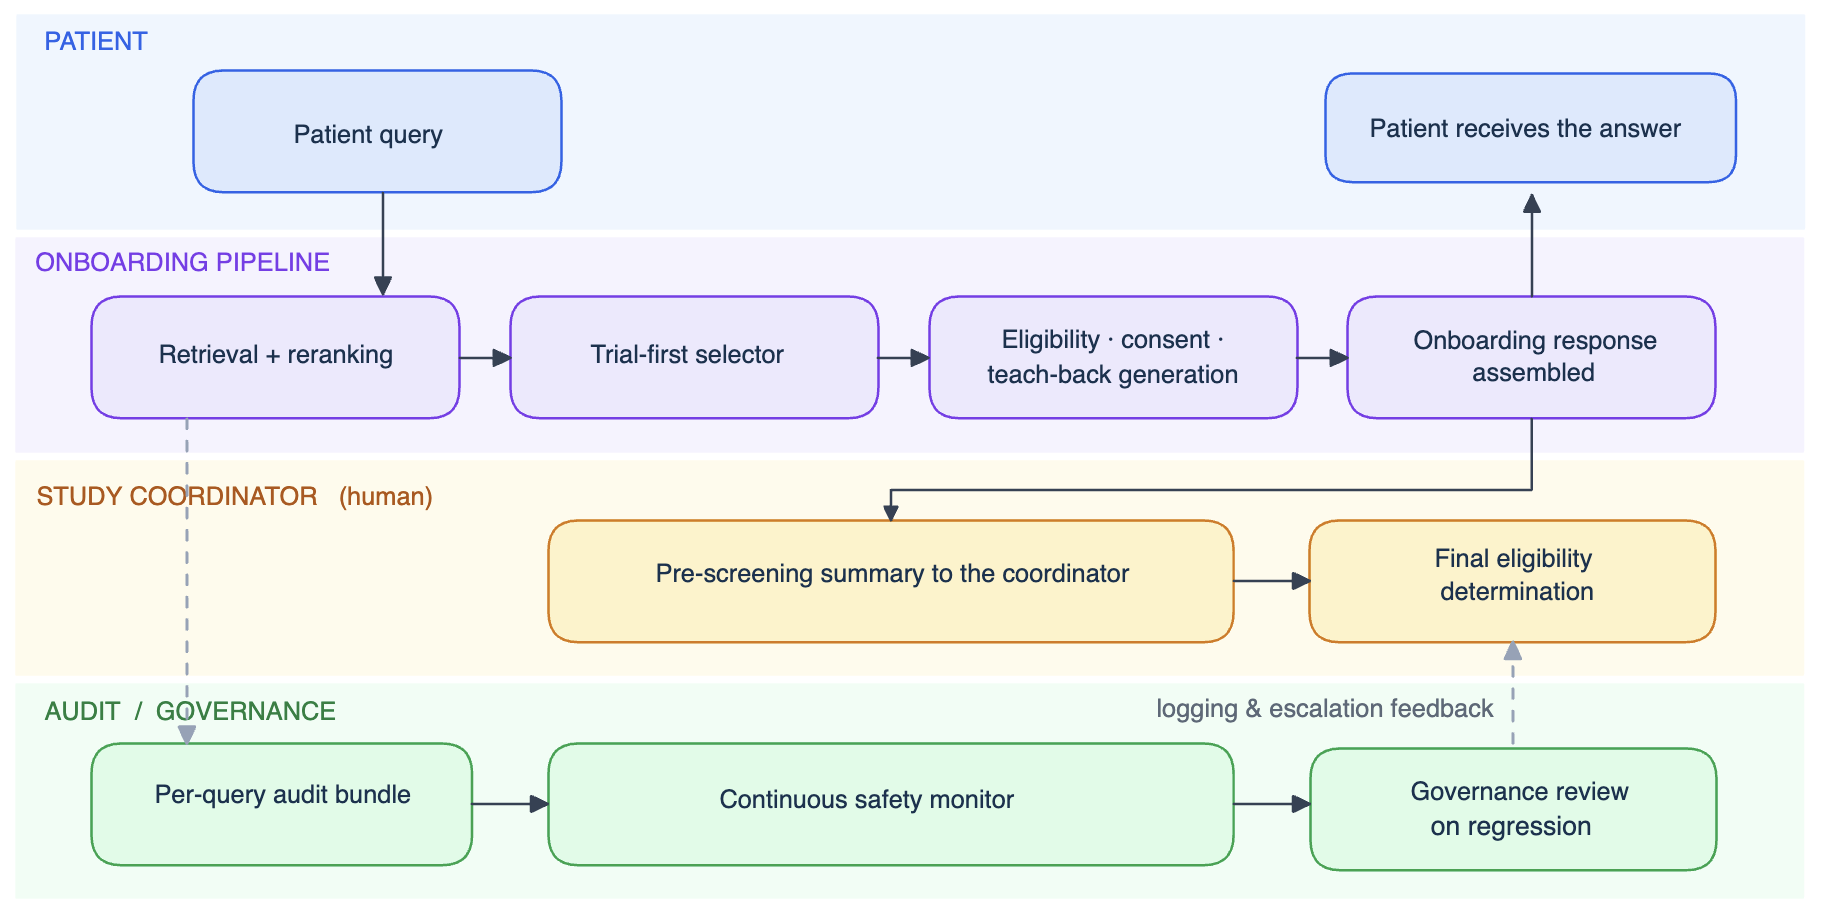
\includegraphics[width=0.96\linewidth]{figures/deployment_workflow.png}
\caption{\textbf{Clinical deployment workflow with four roles.} Patient, automated pipeline, study coordinator, and audit / governance layer. The pipeline is a pre-screening clarification aid; the final eligibility decision remains with the study team. Audit JSON is persisted per query; the continuous safety monitor watches leak / parse-fail / over-abstain rates and triggers governance review on regression.}
\label{fig:deployment}
\end{figure}

\paragraph{Representativeness of the case pool.}
The evaluation pool of $n=114$ cases combines (i) 50 TREC Clinical Trials topics drawn from the 2021 and 2022 judged pools \citep{roberts2021trec,soboroff2022trec}, (ii) 22 surface-form paraphrases of the curated 30-case audit corpus, (iii) 12 hand-crafted vague queries that the deployed system should refuse to anchor, and (iv) the original 30 anchor cases spanning seven intent categories (anchor / partial / mismatch / explanation / participation / risk / consent). The TREC topics are peer-reviewed gold-standard IR benchmarks used by multiple trial-matching papers; the six therapeutic-area strata (musculoskeletal, cardiovascular, metabolic, oncology, neurology / CNS, and a heterogeneous \emph{Other} bucket) cover the bulk of US active-trial volume reported in ClinicalTrials.gov. We do not claim universal representativeness---no single 114-case pool can---but the pool spans both selector regimes (32 accept, 82 abstain), seven intent categories, and six therapeutic areas, a coverage profile that the prior trial-matching evaluations cited above do not report. The full provenance manifest is released for re-stratification by other groups (Supplementary Table~S4).

\paragraph{Limitations.}
We highlight six. \emph{(i) Rubric-and-rater design.} The 15-case ablation contrasting the unconstrained, strict-abstain, and final guarded variants is single-rater; we triangulate against two independent LLM judges and reach moderate agreement on the V1 stratum where the rubric retains variance, but a multi-rater clinician audit is deferred to follow-up work. The present study is therefore best interpreted as a pre-clinical technical audit of a specific safety failure mode (cross-trial conflation), not as evidence of patient comprehension or clinical effectiveness. We exclude human-subject evaluation at this stage by design: under early-stage clinical-AI staging \citep{vasey2022decideai}, a technical safety audit that closes the dominant failure channels is the ethical prerequisite for exposing patients or clinical staff to the system---not a substitute for the human evaluation it enables. \emph{(ii) Empirical coverage of the audited regime.} The zero-lexical-leak result is reported as an empirical bound over six model families, six therapeutic areas, two selector regimes, and one institutional cohort---not a general guarantee. Deployment in a new institution, a new backbone family, or under-represented populations \citep{unger2019recruitment,clark2019barriers,fda2022diversity,chang2024fair} (pediatrics, rare disease, non-English) should replicate the dual-leak audit and per-gate ablation on local queries before going live. Algorithmic-fairness audits should also accompany any deployment that uses local enrollment records, since equity failures of healthcare ML have been documented when training pipelines fail to account for population structure \citep{obermeyer2019dissecting}. \emph{(iii) Clinical-utility validation.} Utility rests on LLM-judge rubric scores rather than patient-perceived comprehension; a human-subject teach-back study is required for full clinical-utility validation. \emph{(iv) Calibration.} The selector score share $\tau$ has a negative Brier Skill Score against held-out relevance targets and is unsuitable as a per-case triage probability; we recommend using only the binary accept/abstain flag in patient-facing UI and treating $\tau$ drift as an internal monitoring signal. \emph{(v) Human evaluation is LLM-judge-based pending independent clinical review.} The headline safety and utility signals rest on two LLM judges; we have prepared a blinded clinical-expert review packet (Methods, \S\ref{sec:methods_expert}) and recruitment through clinical collaborators is in progress, with independent-reviewer results to be incorporated prior to publication. Until then, the LLM-judge findings should be read as a pre-clinical technical audit. \emph{(vi) Residual semantic channel is reduced but not eliminated.} The claim-level NLI verifier (\S\ref{sec:results_nli}) redacts $8$ of the $12$ both-judges-consensus semantic leaks---the eight manual review classifies as genuine cross-trial content---at a $15.1\%$ per-claim utility cost, and is the recommended deployment hardening for the smallest backbone where the residual concentrates. It does not remove generator-level T2 unsupported-completion errors, and its utility cost argues for selective application (e.g., on the adversarial subset, $\rho<1.5$) rather than globally; tuning the redaction margin and entailment model is left to deployment-time calibration.

% ============================================================
\section{Methods}
\label{sec:methods}

\subsection{Problem formulation and operational definitions of leakage}
\label{sec:methods_leak_def}
A clinical trial onboarding instance is a tuple $(q, \mathcal{P})$ where $q$ is a patient utterance and $\mathcal{P} = \{p_1, \ldots, p_m\}$ is a set of candidate trial passages. Let $\mathcal{T}$ denote the distinct \texttt{NCT}-indexed trials in $\mathcal{P}$. The system produces four structured outputs: (i) an evidence set $E \subseteq \mathcal{P}$; (ii) an eligibility assessment $A = (d, F^+, F^-, R^-)$ with conservative decision $d \in \{\emph{LM}, \emph{PMIE}, \emph{LMM}, \emph{CD}\}$; (iii) a consent-style explanation $C$ whose fields either cite evidence or default to the fallback string \fallback; (iv) a teach-back set $T$ of clarification questions conditioned on $F^-$ and $R^-$. A response \emph{leaks} when it references a trial other than $t^\star$, the trial accepted by the selector. We pre-specified three complementary detectors: (a) \textbf{narrow leak}: any \texttt{NCT$\backslash$d$\{8\}$} regex match other than $t^\star$ in the union of model-emitted text fields after lower-casing and whitespace stripping; (b) \textbf{wide (entity-resolved) leak}: narrow leak \emph{or} any token from $\bigcup_{t \neq t^\star} V(t)$, where $V(t)$ is the set of length-$\geq 6$ alphabetic title tokens unique to trial $t$ in the corpus, after removing a curated stop-list of generic clinical English (\texttt{study, trial, patient, treatment, \ldots}; full list in Supplementary \S2.5); (c) \textbf{semantic leak (LLM-judge)}: paraphrased factual content (eligibility criterion, dose, schedule, procedure, sponsor detail) that is supported only by some non-selected trial $t \neq t^\star$ in the retrieval pool. Two independent judges (Claude Sonnet~4.5 and GPT-4o) score every generation blindly against the selected-trial passages and the top-$k$ non-selected candidate passages and return a binary flag, the suspect $t$, a $\leq 250$-char claim excerpt, and a rationale (prompt + per-case audit in Supplementary \S2.6). The headline rate we report is the conservative \emph{both-judges-agree} consensus; the per-judge marginals and the either-judge rate are reported alongside. The narrow and wide detectors are computed deterministically from persisted JSON; the semantic detector is logged with per-call latency, retry count, and full prompt for reproducibility.

\subsection{Trial-first single-context selector}
The selector accepts a single dominant trial only if four numerical signals clear deployment thresholds and a generic-question heuristic does not fire. For each distinct trial $t$ we compute a trial-level score $S(t) = \sum_{p \in \mathcal{E},\, \mathrm{doc}(p)=t} \sigma(s(p))$, where $s(p)$ is the cross-encoder score and $\sigma$ is a clipped softplus. Let $t^\star = \arg\max_t S(t)$ and $t^{(2)}$ the runner-up. We compute four signals: dominance ratio $\rho = S(t^\star)/\max(S(t^{(2)}), \epsilon)$; trial-score share $\tau = S(t^\star)/\sum_t S(t)$; raw maximum cross score $\mu = \max_{p:\mathrm{doc}(p)=t^\star} s(p)$; and best rank $\kappa$. The context is accepted iff $\rho \ge \rho_{\min}$, $\tau \ge \tau_{\min}$, $\mu \ge \mu_{\min}$, $\kappa \le \kappa_{\max}$, and the generic-flag $g$ does not fire. Deployed thresholds: $(\rho_{\min}, \tau_{\min}, \mu_{\min}, \kappa_{\max}) = (1.35, 0.28, -4.5, 2)$ with $k_{\text{keep}}=6$ accepted passages; the negative floor on $\mu_{\min}$ reflects that $s(p)$ is a raw pre-sigmoid cross-encoder logit and therefore takes values in $\mathbb{R}$, with $-4.5$ chosen to exclude only the lowest-confidence reranker outputs while admitting moderately ranked but plausible top passages. The generic-flag is a deterministic 21-phrase substring detector validated at precision 0.75 / recall 0.86 on the 15-case audit pool (Supplementary \S2.5; full trigger list in Supplementary Table~S3). Pseudocode for the selector and the downstream guarded eligibility, strict consent, and teach-back modules is in Supplementary \S2.

\subsection{Case-set construction and representativeness}
\label{sec:methods_cases}
The $n=114$ pool combines the curated 30-case audit corpus (selector-accept regime; covers seven patient-facing intent categories from the trial-matching literature) with an 84-case extension built from (i) 50 TREC CT 2021 / 2022 topic IDs drawn stratified across area and topic length and minimally rewritten from third-person clinical sketches into first-person patient-facing questions (e.g., ``A 50-year-old man with non-Hodgkin lymphoma\ldots'' $\to$ ``I am a 50-year-old man with non-Hodgkin lymphoma\ldots''); (ii) 22 surface-form paraphrases of curated cases; and (iii) 12 hand-crafted vague queries (``I had some bone problems'') that the deployed system should refuse to anchor. Each case carries a gold \texttt{NCT} (where applicable), an intent category, and an LLM-assigned therapeutic-area label that was manually spot-checked. Area distribution: 14 / 8 / 19 / 16 / 13 / 44 across MSK\_Bone / Cardiovascular / Metabolic\_Endocrine / Oncology / Neurology\_CNS / Other. Cases with no clearly dominant trial in the candidate pool are tagged \emph{selector-abstain expected}; cases with a clear dominant trial are tagged \emph{selector-accept expected}. The deployed thresholds match this expected behavior on approximately $78\%$ of cases; the disagreements are dominated by selector-conservative behavior on borderline accepts. Linkage between the 15-case ablation pool (used in Supplementary \S3 to compare V1 / V2 / V-final variants on a ten-dimension human rubric) and the $n=114$ safety pool (used here for the headline claim) is documented in Supplementary \S2.6: the 15-case audit is the qualitative-design study; the $n=114$ pool is the safety-claim study; both are released.

\subsection{Per-gate counterfactual ablation}
\label{sec:methods_pergate}
For each gate $X \in \{\rho, \tau, \mu, \kappa, \mathrm{generic}\}$, we define a variant \emph{V-final-no-}$X$ that drops gate $X$ while keeping the others. Because the broader 84-case pool was generated with the gate disabled, the leak / commit / abstain rates per (variant, backbone) are computed from the existing JSON records without any new inference. The full per-variant accepted-case lists are released as Supplementary Data.

\subsection{Baseline configurations}
\label{sec:methods_baselines}
Four baselines were pre-registered in a frozen configuration file (committed before any baseline generation) and run on the two deployment backbones (Qwen-2.5-7B-Instruct, Qwen-2.5-3B-Instruct) over the same $n=114$ pool, holding retrieval, the JSON-schema prompt scaffold, and the post-processor identical to V-final and varying only the evidence-control mechanism. \textbf{B1 (multi-trial RAG)}: the top-$6$ reranked passages across all pool trials are passed to the generator with no single-trial guard. \textbf{B2 (prompt-only guard)}: the same multi-trial evidence plus a strong anti-mixing system instruction (frozen verbatim in the configuration: identify the single most relevant trial and answer only from it; never combine details across trials; otherwise ask for the study title or \texttt{NCT} number). \textbf{B3 (citation-enforced)}: the same multi-trial evidence with a schema requiring \texttt{support\_passages} identifiers for every narrative field; fields without valid citations are dropped to the fallback string. \textbf{B4 (top-1 selection)}: the trial owning the rank-1 passage is accepted unconditionally (the trivial structural guard), bypassing the five-gate ensemble but retaining the downstream guarded modules. For B1--B3 the reference trial against which the leak detectors evaluate ``other-trial'' content is the rank-1 passage's trial. All $912$ baseline generations are audited by the identical narrow, wide, and dual-judge semantic detectors used for V-final, and scored on the five-dimension rubric.

\subsection{Failure taxonomy}
\label{sec:methods_taxonomy}
Every consensus-flagged generation is classified into three mutually exclusive categories. \textbf{T1 (cross-trial contamination)}: the erroneous claim is supported only by a non-selected trial present in the retrieval pool---i.e., information fused from a different study. \textbf{T2 (unsupported clinical completion)}: plausible protocol-style content supported by no trial in the pool, generated from parametric memory. \textbf{T3 (ordinary hallucination)}: a claim false on its face or incoherent with the case, not attributable to any trial. The distinction is operationalized in the dual-judge semantic prompt, which returns a taxonomy label alongside the binary leak flag; the author adjudicated the consensus-flagged cases. T1 is the evidence-layer failure mode the pipeline is designed to eliminate; T2/T3 are generator-level errors that single-trial control is not expected to remove.

\subsection{Claim-level NLI verification}
\label{sec:methods_nli}
The claim-level verifier scores each asserted patient-facing claim with a natural-language-inference model (\texttt{MoritzLaurer/DeBERTa-v3-large-mnli-fever-anli-ling-wanli}). For a claim $c$, it computes $e_{\mathrm{sel}}(c)$, the maximum entailment probability over the selected trial's passages, and $e_{\mathrm{other}}(c)$, the maximum over any non-selected pool trial's passages (premises chunked to the model's input limit). A claim is redacted iff $e_{\mathrm{other}}(c) \ge \tau_{\mathrm{NLI}}$ \emph{and} $e_{\mathrm{other}}(c) > e_{\mathrm{sel}}(c)$---the operational definition of T1 cross-trial contamination. Single-trial-evidence outputs have no non-selected premise and are therefore never modified by construction. The threshold was calibrated on the 15-case development pool alone, choosing the highest $\tau_{\mathrm{NLI}}$ whose benign-claim drop rate stayed $\le 10\%$ ($\tau_{\mathrm{NLI}}=0.95$; development benign-drop $8.8\%$); the value was fixed before any application to the audit pool, and the counterfactual audit reapplies the frozen verifier to all 684 deployed and 912 baseline generations.

\subsection{Independent clinical-expert review protocol}
\label{sec:methods_expert}
To complement the LLM-judge evaluation with independent clinical judgment, we prepared a blinded expert-review packet of 30 generations stratified across selector regime (accept/abstain), semantic-flag status, and backbone, with the deployed pipeline and two contrast baselines (B1, B4). Each case is presented as a de-identified dossier (patient question, the trial passages shown to the system, and the full patient-facing response) under a randomized, blinded identifier with no model name. Reviewers score each case on the same five-dimension rubric used by the LLM judges plus a binary cross-trial-leak judgment and a T1/T2/T3 taxonomy label, and may add free-text comments. Expert--LLM-judge agreement (Cohen's $\kappa$, Spearman $r_s$) and the expert leak rate with Clopper--Pearson intervals are computed by a released analysis script. All queries are synthetic and contain no patient data; the packet and scoring instrument are released. Reviewer recruitment through clinical collaborators is in progress, and the independent-review results will be added prior to publication.

\subsection{Blind dual-judge LLM evaluation and blinding mechanics}
\label{sec:methods_judge}
Two LLM judges (Claude Sonnet~4.5 and GPT-4o) blind-scored each generation on five integer dimensions (factuality, groundedness, abstention appropriateness, safety, patient utility; 1--5). Blinding was implemented as follows: each $(\text{case}, \text{backbone})$ pair was assigned a stable identifier $\texttt{blind\_id} = \mathrm{SHA1}(\texttt{phase3:case\_id:backbone})[:12]$ that the judge prompt referenced as the only handle; the prompt called the response \emph{Assistant response} with no model name; case order was independently shuffled per judge with different random seeds; and judges received the postprocessed JSON output (a normalized schema-validated object) rather than the raw decoder text, removing model-specific verbose styles that could leak backbone identity. We also stripped any backbone-name occurrence from the served context and rejected (re-served) any case where a parse-extracted field literally matched a known backbone name. Per-dimension Cohen's $\kappa$ \citep{cohen1960kappa,landis1977kappa} at linear and quadratic weights, two-way random intraclass correlation coefficient ICC(2,1), Spearman rank correlation $r_s$, exact-match rate, and mean absolute delta are reported in Supplementary Table~S8; Krippendorff's $\alpha$ at the interval level \citep{krippendorff2018content,hayes2007krippendorff} for the 3-rater (Human + Sonnet + GPT-4o) audit is in Supplementary Table~S9.

\subsection{Retrieval, generation backbones, and audit artifacts}
\label{sec:methods_misc}
Retrieval used a two-stage \textsc{BM25} full-text $\to$ cross-encoder reranker on the TREC CT 2021 corpus \citep{roberts2021trec,robertson2009bm25,nogueira2019passage,hofstatter2021crossenc,lin2021pyserini}; dense alternatives based on Sentence-BERT \citep{reimers2019sbert} and contrastive contriever pretraining \citep{izacard2022contriever}, along with BEIR-style zero-shot retrieval evaluation \citep{thakur2021beir}, were considered as fallbacks but produced no measurable safety gain on this corpus (Supplementary Table~S14). The four open-weight backbones were Qwen-2.5-3B-Instruct (deployment candidate), Qwen-2.5-7B-Instruct, Meta-Llama-3.1-8B-Instruct, and Mistral-7B-Instruct-v0.3 \citep{qwen25_2024,touvron2023llama2}; the two zero-shot closed-API baselines were GPT-4o (\texttt{temperature=0.0}, \texttt{max\_tokens=1500}) and Claude Sonnet~4.5. All six models share the same retrieval, reranker, selector, postprocessor, and prompt; only the generator changes. Every patient-facing response is accompanied by audit artifacts: (i) the reranked evidence with cross-encoder scores; (ii) the trial-level score table; (iii) the context-selector decision with thresholds; (iv) the raw LLM outputs; (v) the postprocessed JSON. These are persisted per query for downstream review. Retrieval comparison detail (Recall@10 / @20 / @100, normalized discounted cumulative gain (nDCG)@10 / @20 across BM25, dense MiniLM, dense BGE-base, reciprocal rank fusion (RRF), and the two-stage configuration) is in Supplementary Table~S14 and Supplementary Fig.~S13.

% ============================================================
\sloppy
\paragraph{Data availability.} Retrieval experiments use publicly available TREC Clinical Trials 2021 / 2022 data \citep{roberts2021trec,koopman2016trec,soboroff2022trec} and the public ClinicalTrials.gov trial corpus; no patient-identifiable data were collected, processed, or released, and all patient-facing case texts are synthetic. The complete audit bundle generated and analyzed during the current study---per-case evidence CSVs, selector status JSONs, trial-level scores, raw and postprocessed LLM outputs, blinded judge JSON-Lines, per-(case, backbone, judge) rubric scores, the $n=114$ case manifest with provenance tags, the per-gate ablation acceptance lists, the calibration per-bin tables, and the 3-way agreement / Krippendorff $\alpha$ derivations---is publicly available in the GitHub repository at \url{https://github.com/zabirul-islam/clinical-trial-onboarding} and will additionally be archived at Zenodo upon acceptance [persistent DOI to be assigned]. The 660\,MB trial-passage corpus derived from public ClinicalTrials.gov + TREC CT 2021/2022 data is mirrored as a HuggingFace dataset at \url{https://huggingface.co/datasets/zabir1996/clinical-trial-onboarding-corpus} for immediate download. Supplementary Information files included with this article contain the case manifest summary and the inter-rater agreement tables required to interpret the headline results.

\paragraph{Code availability.} The underlying code for this study---retrieval, reranking, trial-first selector ensemble, guarded eligibility / consent / teach-back modules, postprocessor, dual-judge evaluation harness, 3-way inter-rater reliability scripts, per-gate ablation harness, calibration analysis, and the figure-build pipeline---is released under the MIT license at \url{https://github.com/zabirul-islam/clinical-trial-onboarding} and will be archived at Zenodo upon acceptance (DOI to be assigned). The pipeline is local-first and runs on commodity GPU hardware; the deployment-candidate backbone Qwen-2.5-3B-Instruct fits in $<8$ GB of GPU memory.
\fussy

\paragraph{Reproducibility statement.} Every numerical claim in the paper is recoverable from the released artifacts. The selector-signal cache, the per-(case, backbone) generation JSONs, and the dual-judge JSON-Lines are persisted with stable identifiers; re-running the figure scripts on these inputs reproduces the figures byte-for-byte for the deterministic figures and within bootstrap-resample noise for the bootstrapped ones. Re-generation of raw LLM outputs is non-deterministic for closed-API backbones (GPT-4o, Claude Sonnet~4.5); the frozen audit bundle is the canonical reference.

\paragraph{Competing interests.} The authors declare no financial or non-financial competing interests.

\paragraph{Ethics.} This study used only publicly available trial documents and synthetic patient-facing queries. No human subjects were recruited or enrolled, and no IRB approval was required. The system is positioned as a pre-screening clarification aid and is not deployed clinically; in-clinic deployment would require institution-specific IRB review, an updated patient-consent flow for AI-assisted onboarding, and a study-team validation step before any patient sees an output.

\paragraph{Author contributions.} M.Z.I.\ conceived the study, designed and implemented the retrieval / selector / eligibility / consent / teach-back pipeline, ran all experiments, conducted the per-gate ablation and dual-judge audit, performed the inter-rater reliability and calibration analyses, generated the figures and tables, and drafted the manuscript. G.W.\ supervised the project, advised on clinical-safety framing and reporting standards, and critically revised the manuscript. All authors read and approved the final version of the manuscript.

\paragraph{Acknowledgements.} This research received no specific grant from any funding agency in the public, commercial, or not-for-profit sectors. Computational resources were provided by institutional resources of Rensselaer Polytechnic Institute. The authors thank colleagues at Rensselaer Polytechnic Institute for helpful discussions on clinical deployment, audit traceability, and patient-facing language.

% ============================================================
\bibliographystyle{unsrtnat}
\bibliography{references}

\end{document}
